\pagestyle{n-1}
\label{n-1}

\pagebreak


\begin{center}
\hspace*{.5cm}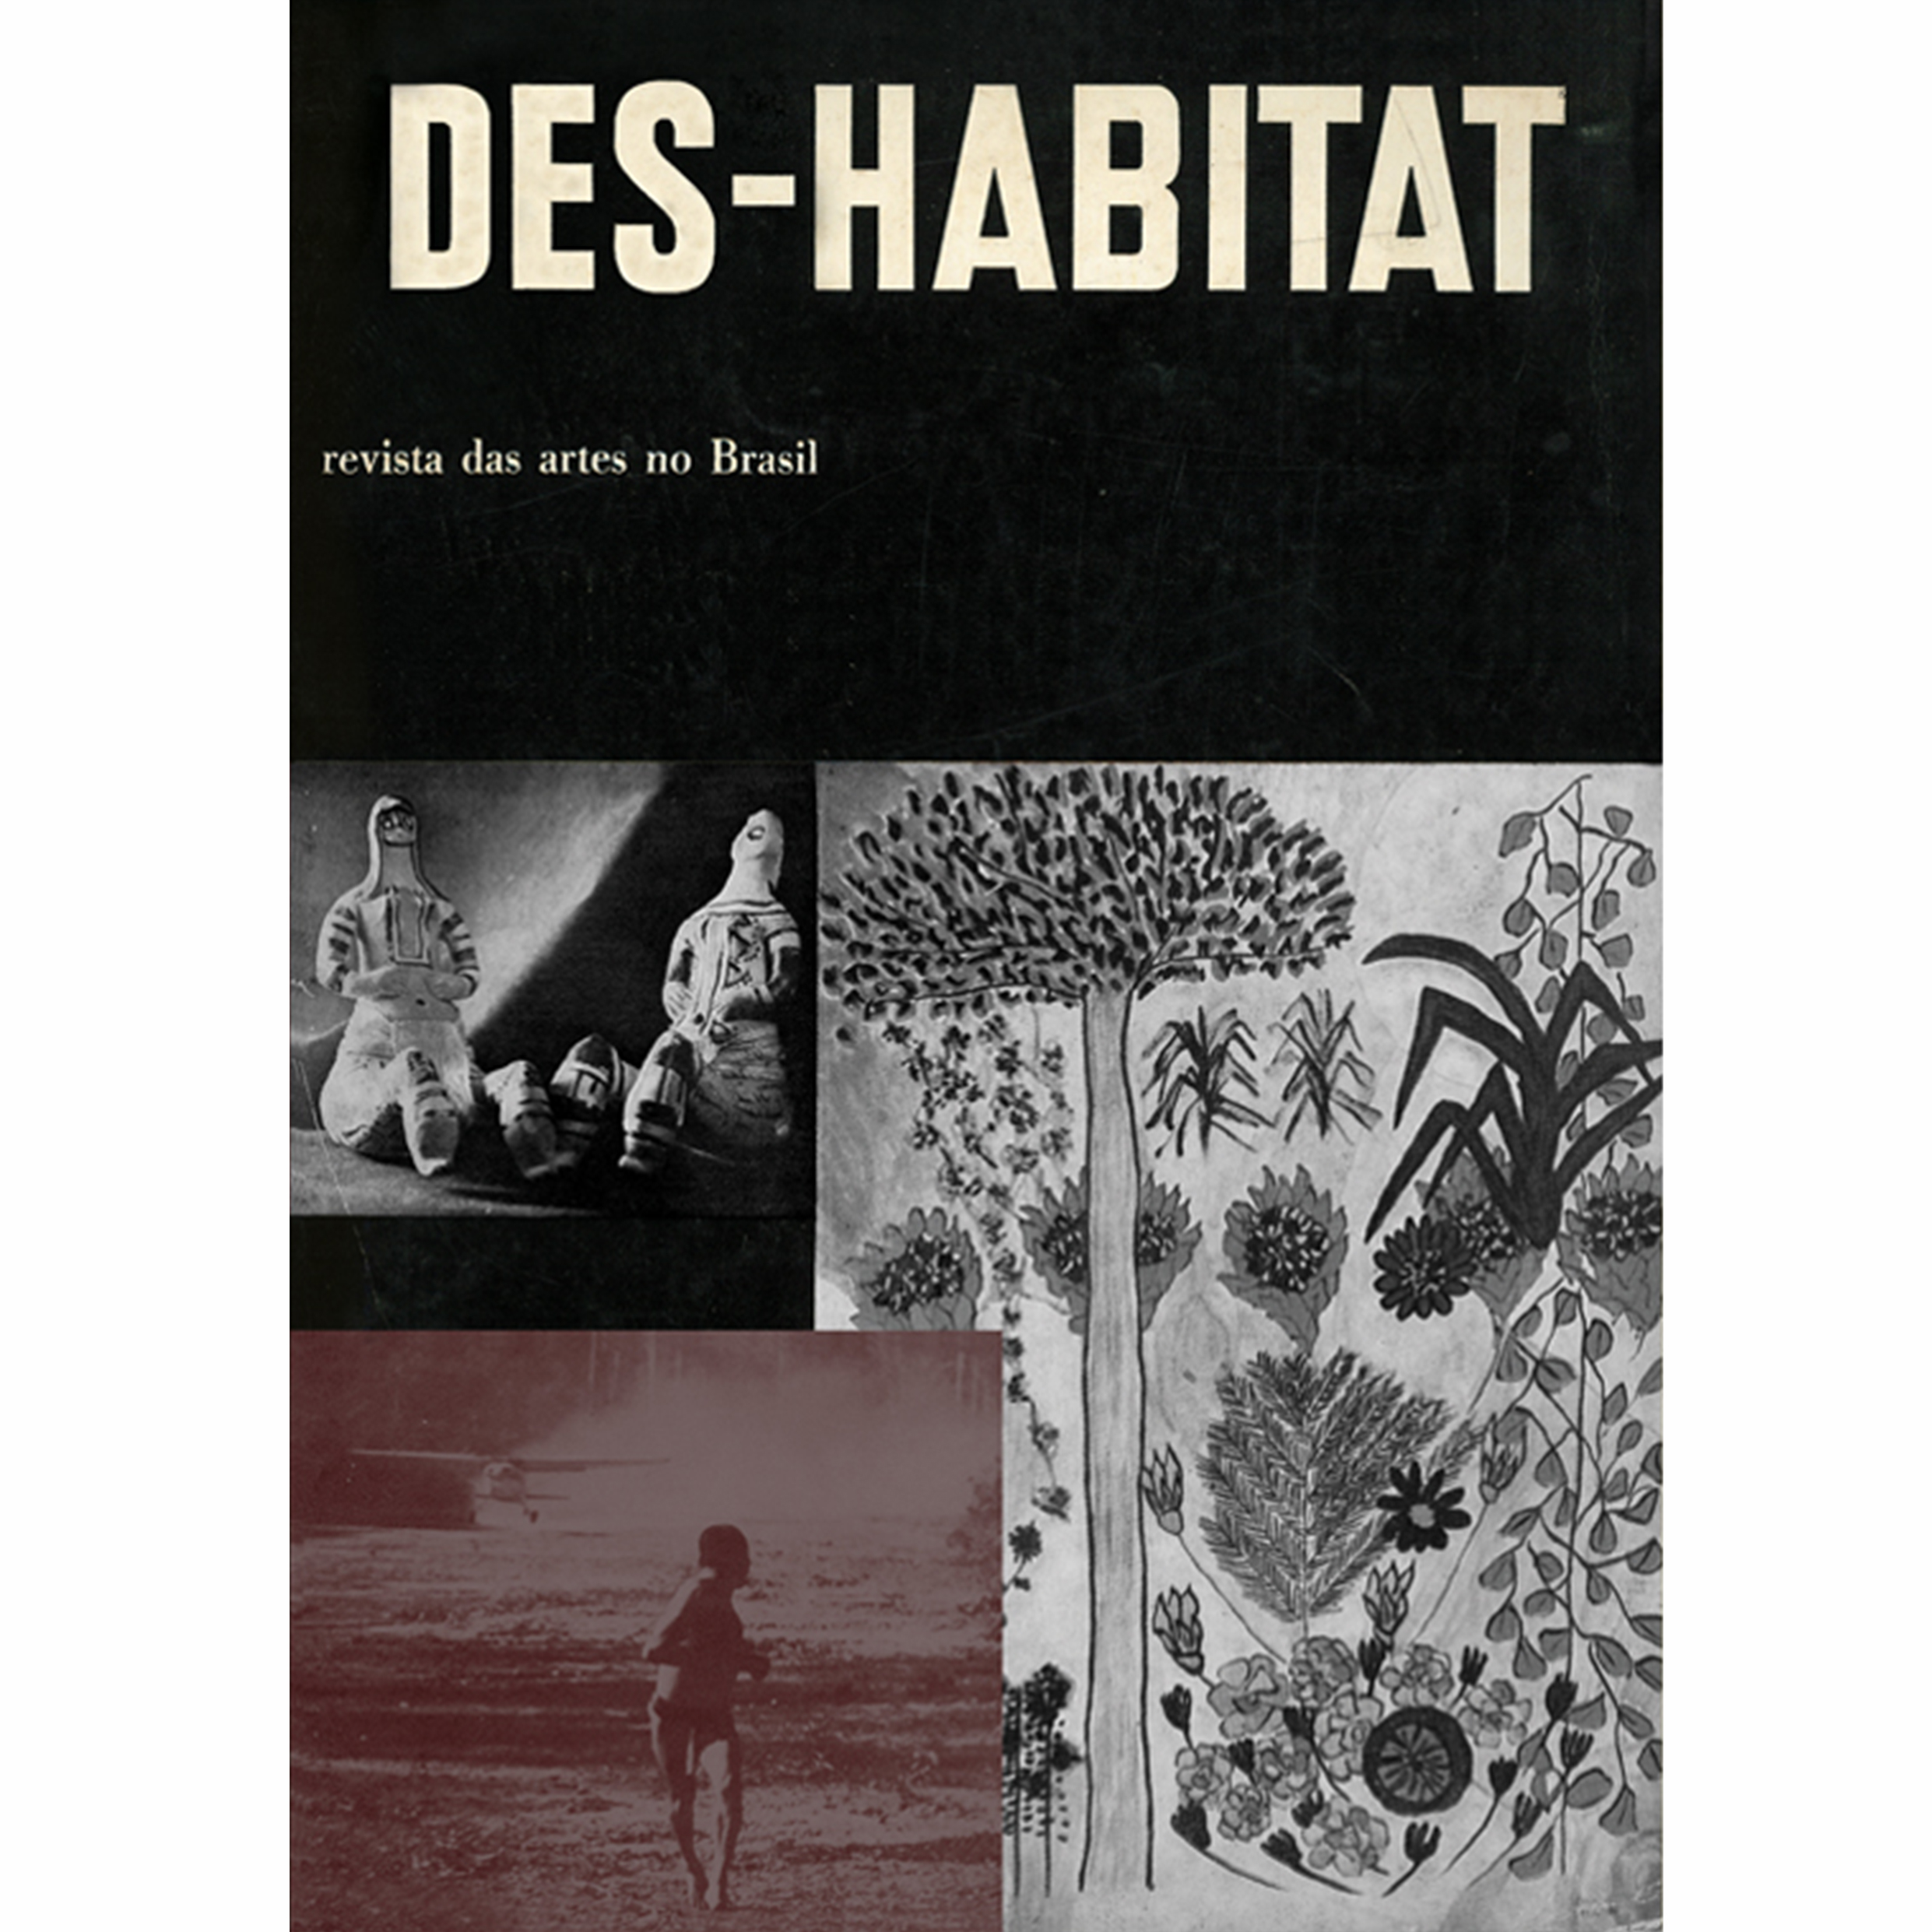
\includegraphics[width=74mm]{./CAPAS/habitat.jpg}
\end{center}

\hspace*{-7cm}\hrulefill\hspace*{-7cm}

\medskip

\noindent{}Neste ensaio visual, Paulo Tavares intervém em \textit{Habitat}, revista de artes e design editada pela arquiteta Lina Bo Bardi nos anos 1950. \hlc{Resignificando imagens e imaginários dominantes, \textit{Des-Habitat} nos carrega através uma narrativa visual sobre a colonialidade da arquitetura moderna e suas mídias}, abrindo um horizonte para a potencial descolonização de seus legados. Com ensaio e design de Paulo Tavares, e prefácio da curadora Marion von Osten, em uma parceria entre agência autônoma e n-1 edições.

\vfill

\hspace*{-.4cm}\begin{minipage}[c]{1\linewidth}
\small\textbf{
\hspace*{-.1cm}Editora: n-1\\
Título: Des-Habitat\\
Autor: Paulo Tavares\\ 
ISBN: 978-65-86941-39-5\\
Páginas: 97\\
Formato: 23,5x33\,cm\\
Preço: R\$ 70,00\\
}
\end{minipage}

\pagebreak %PRAGMATISMO PULSIONAL


\begin{center}
\hspace*{-3.6cm}\raisebox{5cm}{\rotatebox[origin=t]{90}{\huge\textbf{Lançamento}}}
\hspace*{3.1cm}
\includegraphics[width=74mm]{./CAPAS/tempos.jpg}
\end{center}

\hspace*{-7cm}\hrulefill\hspace*{-7cm}

\medskip

\noindent{}Não há tempo moderno, mas tempos modernos, \hlc{maneiras diferentes ou contraditórias de agenciar as temporalidades das artes do movimento}, suas continuidades, seus cortes, seus reajustes e suas retomadas, para produzir obras que respondam às condições do presente e às exigências do futuro.
\vfill

\hspace*{-.4cm}\begin{minipage}[c]{.8\linewidth}
\small\textbf{
\hspace*{-.1cm}Editora: n-1\\
Título: Tempos modernos: arte, tempo, política\\
Autor: Jacques Rancière\\ 
ISBN: 978-65-86941-40-1\\
Páginas: 160\\
Formato: 17x12\,cm\\
Preço: R\$ 65,00\\
}
\end{minipage}

\pagebreak

\begin{center}
\hspace*{.5cm}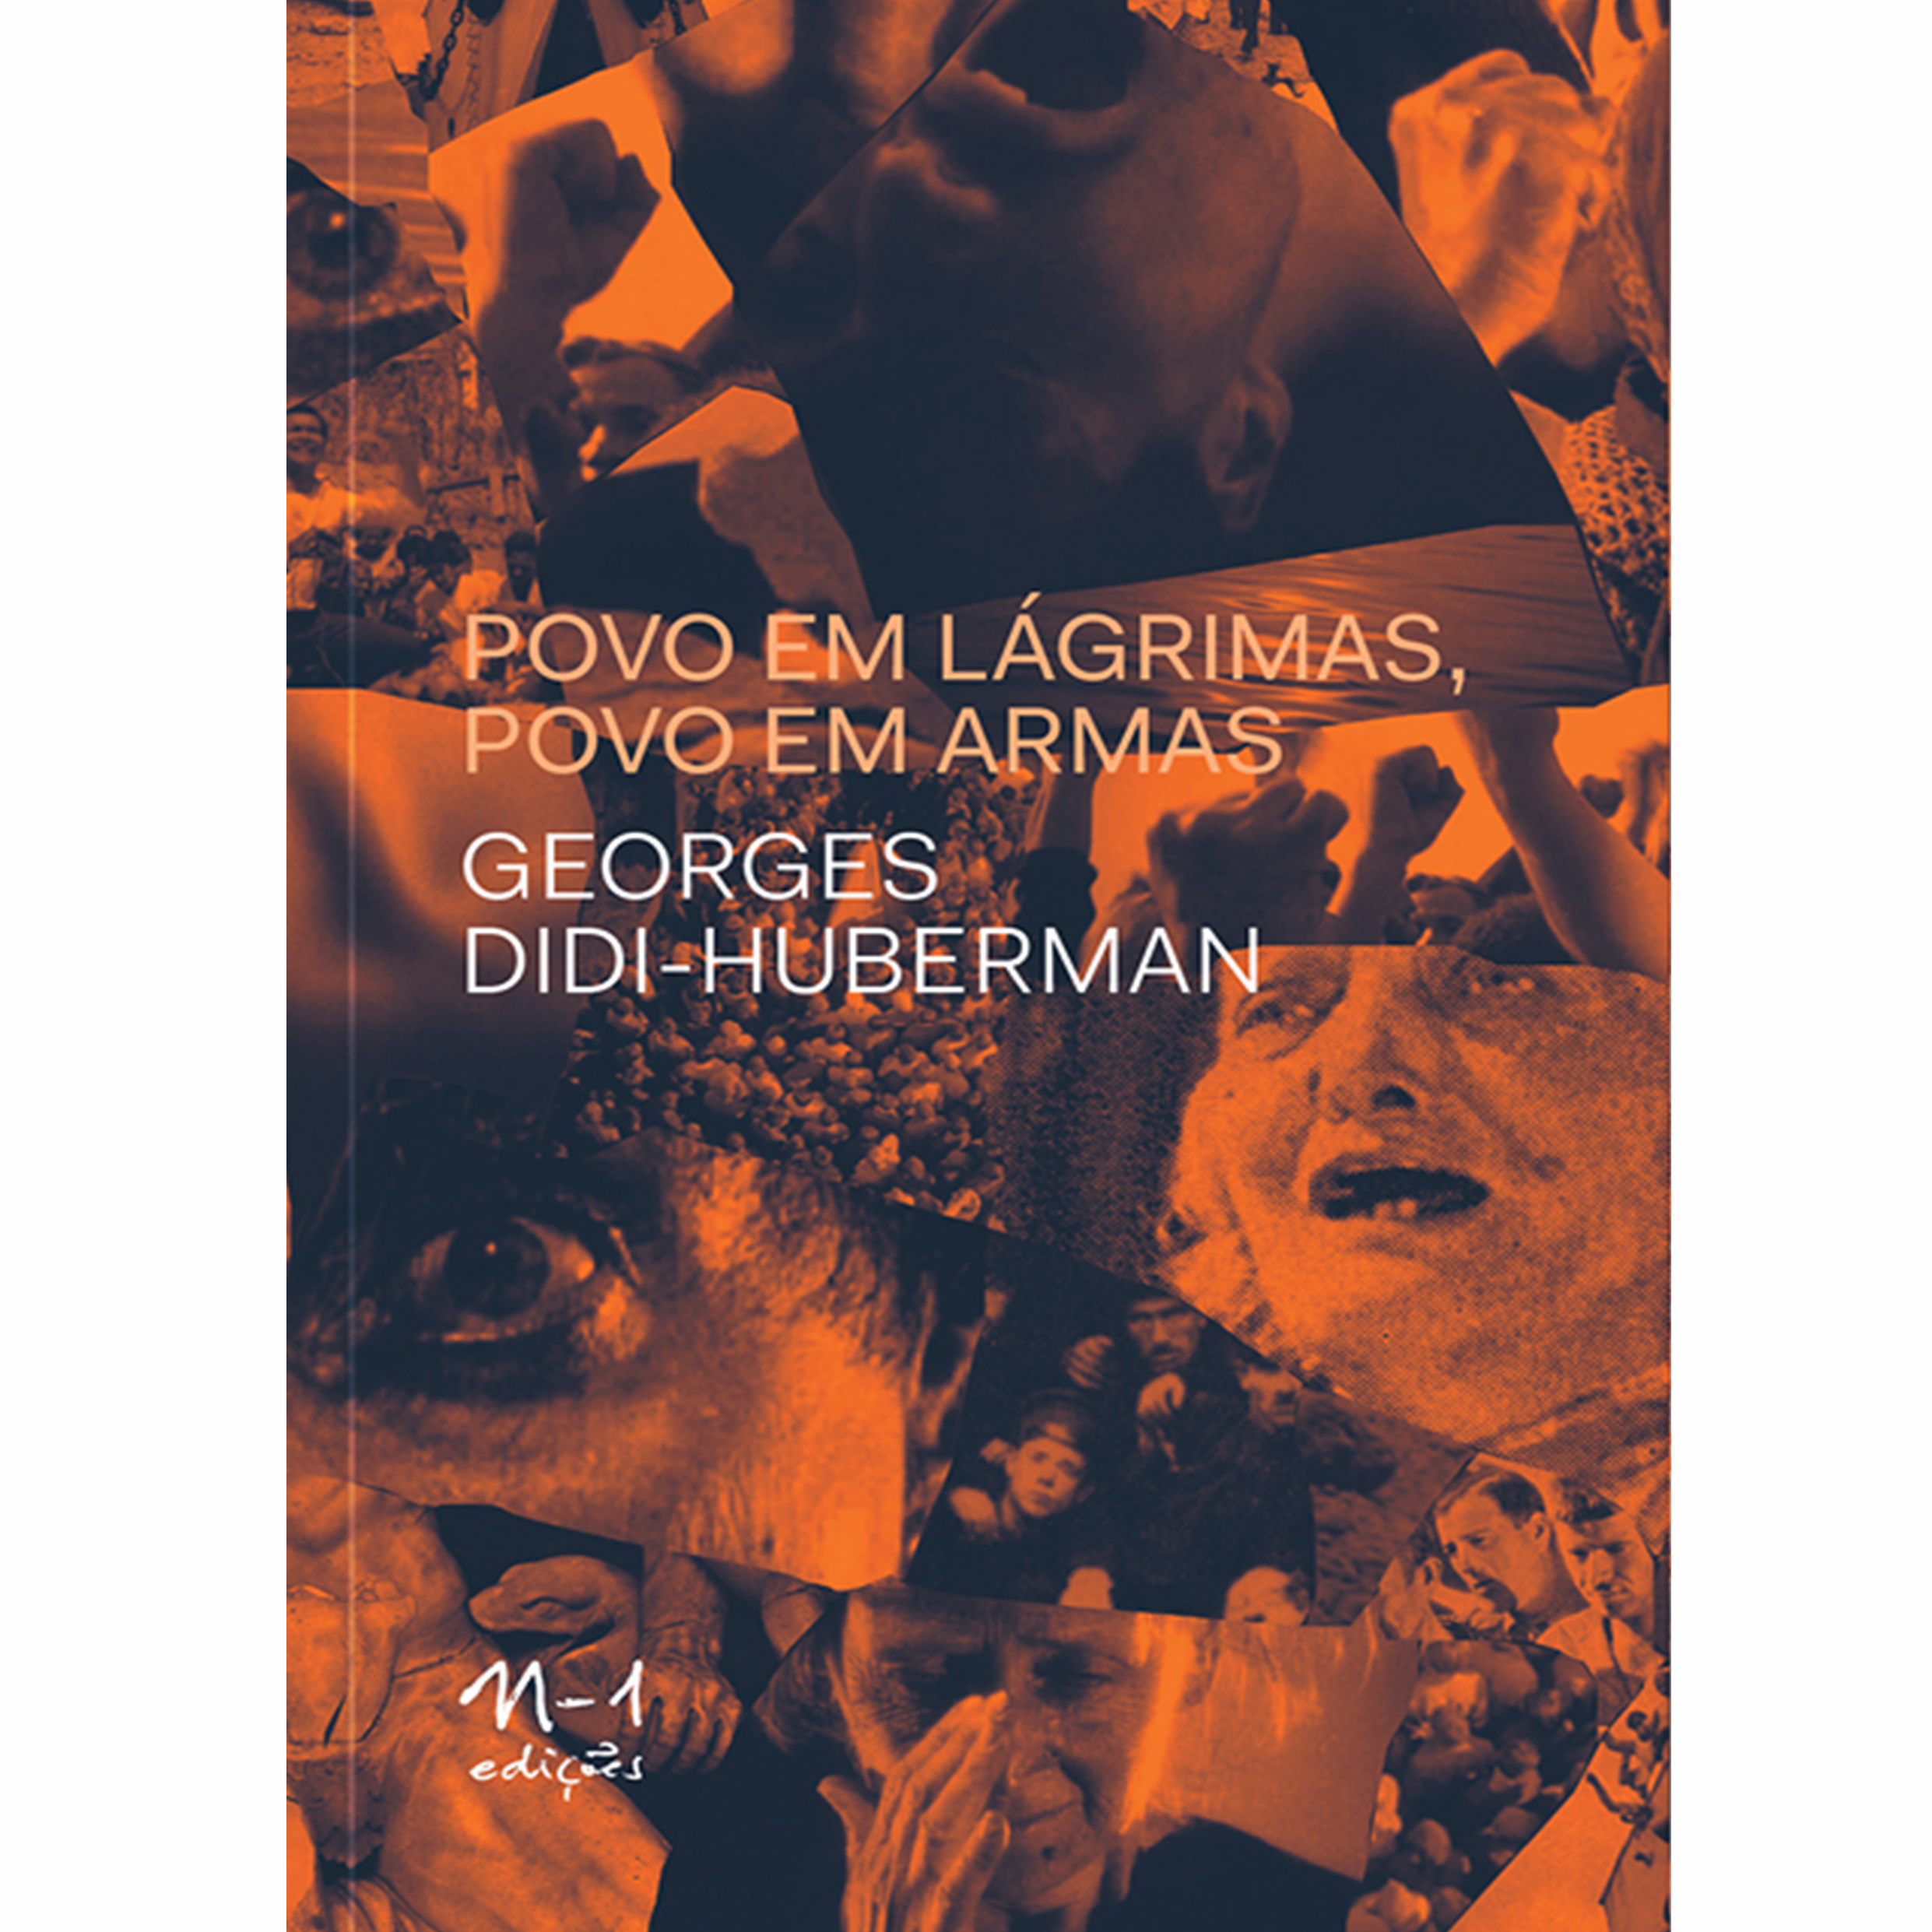
\includegraphics[width=74mm]{./CAPAS/povo.jpg}
\end{center}

\hspace*{-7cm}\hrulefill\hspace*{-7cm}

\medskip

\noindent{}Este livro parte da análise de uma única situação, porém exemplar: um homem morre de morte injusta e violenta; mulheres se juntam para chorá-lo; logo mais é um povo em lágrimas que se reúne a elas. Ora, essa \hlc{situação que se vê por toda parte foi esplendidamente retratada por Serguei Eisenstein em seu célebre filme \textit{O encouraçado Potemkin}. Mas como foi que Roland Barthes, uma das vozes mais influentes no domínio do discurso contemporâneo sobre as imagens, pôde considerar tal construção do \textit{pathos} ``vulgar'' e ``lamentável''?} 
A melhor resposta à crítica \textit{barthesiana} será fornecida pelo próprio Eisenstein na estrutura de sua sequência de imagens, assim como no discurso --- imenso, abundante, genial, tão importante quanto o dos maiores pensadores de seu tempo --- que ele sustenta sobre a questão das imagens patéticas. Descobre-se uma emoção que sabe dizer \textit{nós}, e não só \textit{eu}, um \textit{pathos} que não é apenas passivo, mas se constitui em \textit{práxis}: quando as velhas carpideiras de Odessa, em volta do marinheiro morto, passam da lamentação à cólera, ``prestam queixa'' e exigem justiça, fazem nascer esse \textit{povo em armas} da revolução que vem.

\vfill

\hspace*{-.4cm}\begin{minipage}[c]{.5\linewidth}
\small\textbf{
\hspace*{-.1cm}Editora: n-1\\
Título: Povo em lágrimas, povo em armas\\
Autor: Georges Didi-Huberman\\ 
ISBN: 978-65-86941-18-0\\
Páginas: 520\\
Formato: 14x21\,cm\\
Preço: R\$ 120,00\\
}
\end{minipage}

\pagebreak

\begin{center}
\hspace*{-3.6cm}\raisebox{5cm}{\rotatebox[origin=t]{90}{\huge\textbf{Lançamento}}}
\hspace*{3.1cm}
\includegraphics[width=74mm]{./CAPAS/fabricacao.jpg}
\end{center}

\hspace*{-7cm}\hrulefill\hspace*{-7cm}

\medskip

\noindent{}Ensaio publicado por Heinrich von Kleist em 1870, no qual \hlc{aborda a questão da construção do pensamento durante a fala}. Ensaio crítico introdutório de Maria Cristina Franco Ferraz, onde aponta as conexões deste texto com Nietzsche e a extemporaneidade do pensamento, além do pensamento como máquina de guerra proposto por Deleuze e Guattari. 

\vfill

\hspace*{-.4cm}\begin{minipage}[c]{.5\linewidth}
\small\textbf{
\hspace*{-.1cm}Editora: n-1 \& Hedra\\
Título: Sobre a fabricação gradativa de pensamentos durante a fala\\
Autor: Heinrich von Kleist\\ 
ISBN: 978-65-86941-44-9\\
Páginas: 80\\
Formato: 18x11\,cm\\
Preço: R\$ 36,00\\
}
\end{minipage}

\pagebreak

\begin{center}
\hspace*{.5cm}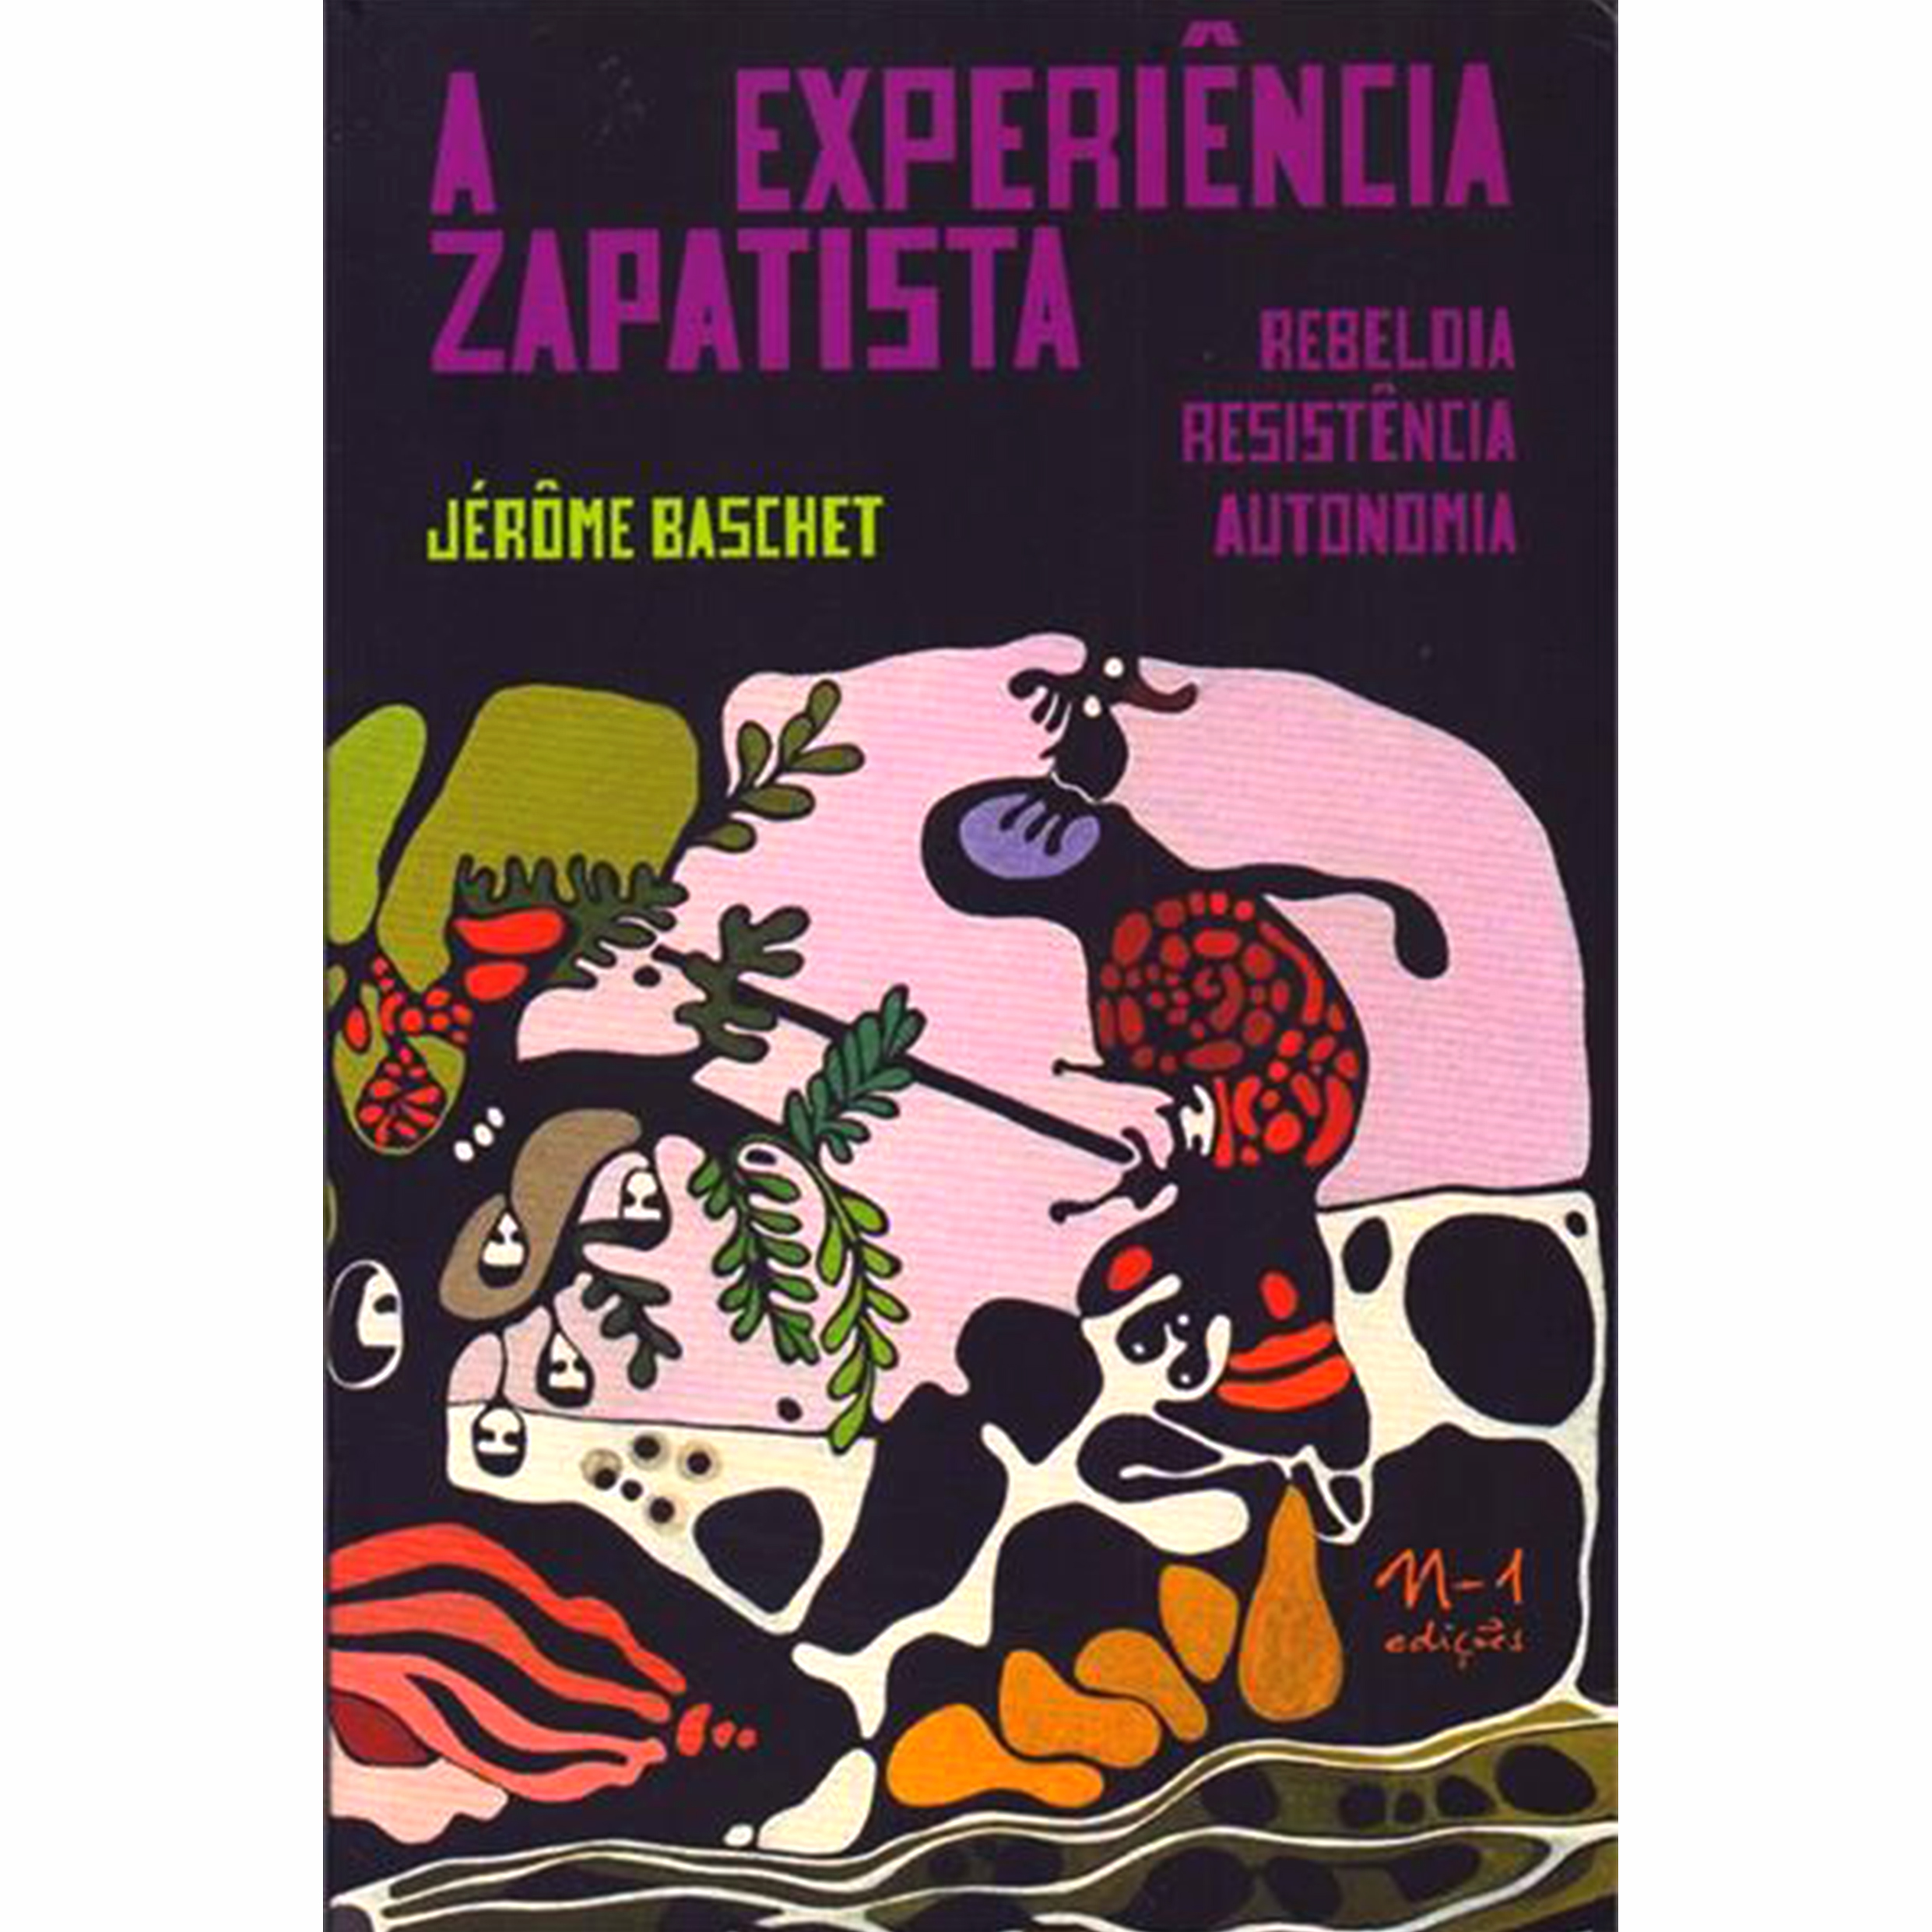
\includegraphics[width=74mm]{./CAPAS/experiencia.jpg}
\end{center}

\hspace*{-7cm}\hrulefill\hspace*{-7cm}

\medskip

\noindent{}``É nossa convicção e nossa prática que para se rebelar e lutar não são necessários nem líderes, nem caudilhos, nem messias, nem salvadores. Para lutar é necessário apenas um pouco de vergonha, um tanto de dignidade e muita organização'', escreveu o Subcomandante Marcos, em 2014. Neste livro, \hlc{o historiador Jérôme Baschet retraça a gênese do movimento zapatista e reconstitui suas várias etapas, desde o levante armado até os dias de hoje}. Assim, temos acesso à lógica de sua organização, à capacidade de autotransformação e à originalidade de sua trajetória. O prefácio do autor acrescido à edição brasileira nos inspira a atravessar a noite tão escura no Brasil à luz da experiência zapatista, que é também indígena, que é também feminina, também poética.

\vfill

\hspace*{-.4cm}\begin{minipage}[c]{.5\linewidth}
\small\textbf{
\hspace*{-.1cm}Editora: n-1\\
Título: A experiência zapatista\\
Autor: Jerôme Baschet\\
ISBN: 978-65-86941-41-8\\
Páginas: 400\\
Formato: 14x21\,cm\\
Preço: R\$ 100,00\\
}
\end{minipage}

\pagebreak

\pagebreak

\begin{center}
\hspace*{-3.6cm}\raisebox{5cm}{\rotatebox[origin=t]{90}{\huge\textbf{Lançamento}}}
\hspace*{3.1cm}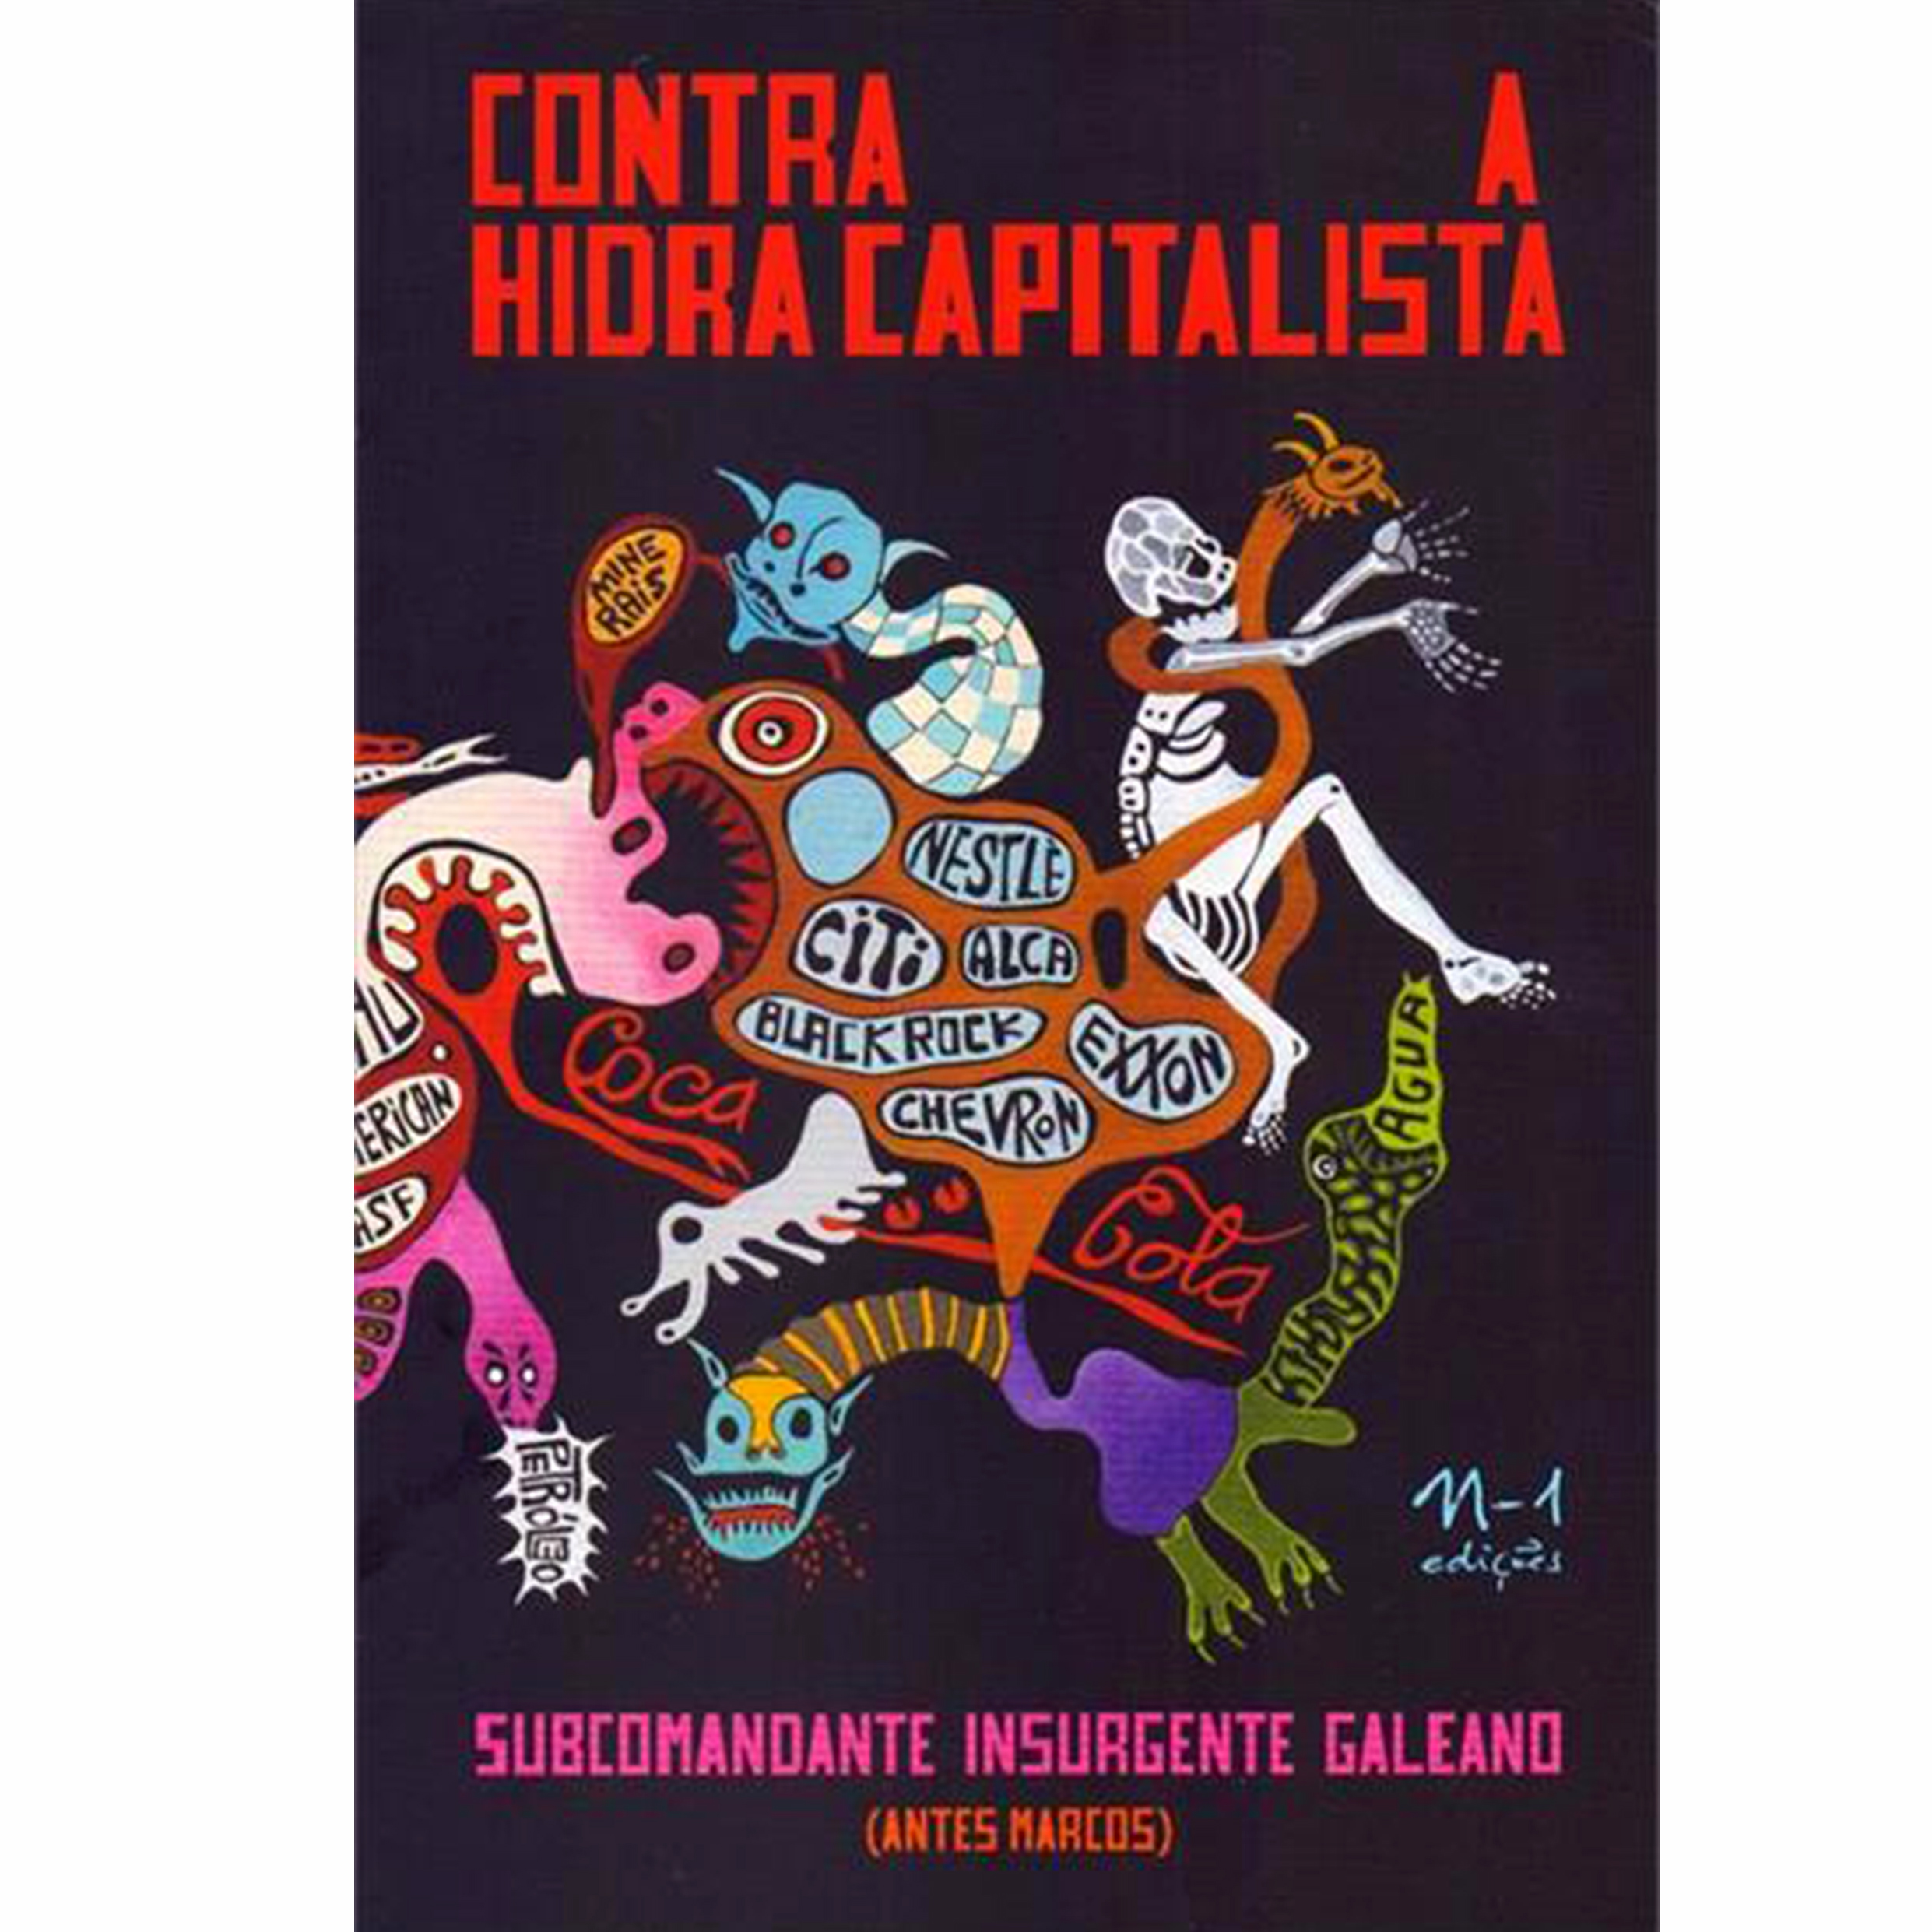
\includegraphics[width=74mm]{./CAPAS/hidra.jpg}
\end{center}

\hspace*{-7cm}\hrulefill\hspace*{-7cm}

\medskip

\noindent{}Para além da aura midiática do encapuzado Subcomandante Insurgente Marcos, rebatizado de Galeano em 2014, \hlc{quase nada sabemos das motivações, aspirações, estratégias e rumos dessa insurgência que desde 1994 ocupa parte do território mexicano. No entanto, ali surgiu um dos bolsões revolucionários mais originais deste século}. Liberados da obsessão estatista, da lógica capitalista, da propriedade privada da terra, da dominação de gênero, de etnia, de classe --- eis uma insurgência que reverteu a mercantilização da existência. Quem melhor do que aquele que a liderou, em seu estilo jocoso, elíptico, à beira da ficção, para dá-la a ver? \textit{Contra a Hidra Capitalista}, com falas do Subcomandante Insurgente Galeano, é um dos quatro livros desta coleção zapatista. Os outros são \textit{A experiência zapatista: rebeldia, resistência e autonomia}, por Jérôme Baschet, \textit{Uma baleia na montanha}, por Mariana Lacerda e Peter Pál Pelbart, \textit{Mensagens revolucionárias}, por Antonin Artaud. As pinturas das capas dos livros são de Rivane Neuenschwander.

\vfill

\hspace*{-.4cm}\begin{minipage}[c]{.5\linewidth}
\small\textbf{
\hspace*{-.1cm}Editora: n-1\\
Título: Contra a hidra capitalista\\
Autor: Subcomandante Marcos Galeano\\ 
ISBN: 978-65-86941-42-5\\
Páginas: 192\\
Formato: 14x21\,cm\\
Preço: R\$ 70,00\\
}
\end{minipage}

\pagebreak

\begin{center}
\hspace*{.5cm}\includegraphics[width=74mm]{./CAPAS/devir.jpg}
\end{center}

\hspace*{-7cm}\hrulefill\hspace*{-7cm}

\medskip

\noindent{}Itziar Ziga conhece a cidade como quem sempre viveu fora. Anda pelas ruas como se pertencessem a ela. Sapatos de princesinha, mas com as solas desgastadas. Dá pra perceber que já fez todos os trajetos, tanto de noite quanto de dia, tanto alerta quanto doidona, com os olhos cheios de lágrimas ou de raiva, em grupo, casal, trisal, sozinha, mas sempre parte da matilha. Mulher da rua, garota de bar, rata de livrarias e corredora de manifestações. \hlc{Itziar Ziga é uma mistureba político-cultural: o campo e a cidade, sua mãe e suas colegas, Euskalerria e Catalunya, o melô e o feminismo iraquiano, Judith Butler e Manuela Trasobares, a teoria queer e as oficinas de pantojismo, a cultura trans e as avós putas, Alaska e Benedetti, santa Ágata e a Dulce Neus}. (Trecho do prefácio de Paul B. Preciado e Virginie Despentes)

\vfill

\hspace*{-.4cm}\begin{minipage}[c]{.5\linewidth}
\small\textbf{
\hspace*{-.1cm}Editora: n-1\\
Título: Devir cachorra\\
Autor: Itziar Ziga\\
ISBN: 978-65-86941-47-0\\
Páginas: 176\\
Formato: 14x21\,cm\\
Preço: R\$ 54,00\\
}
\end{minipage}

\pagebreak

\begin{center}
\hspace*{-3.6cm}\raisebox{5cm}{\rotatebox[origin=t]{90}{\huge\textbf{Lançamento}}}
\hspace*{3.1cm}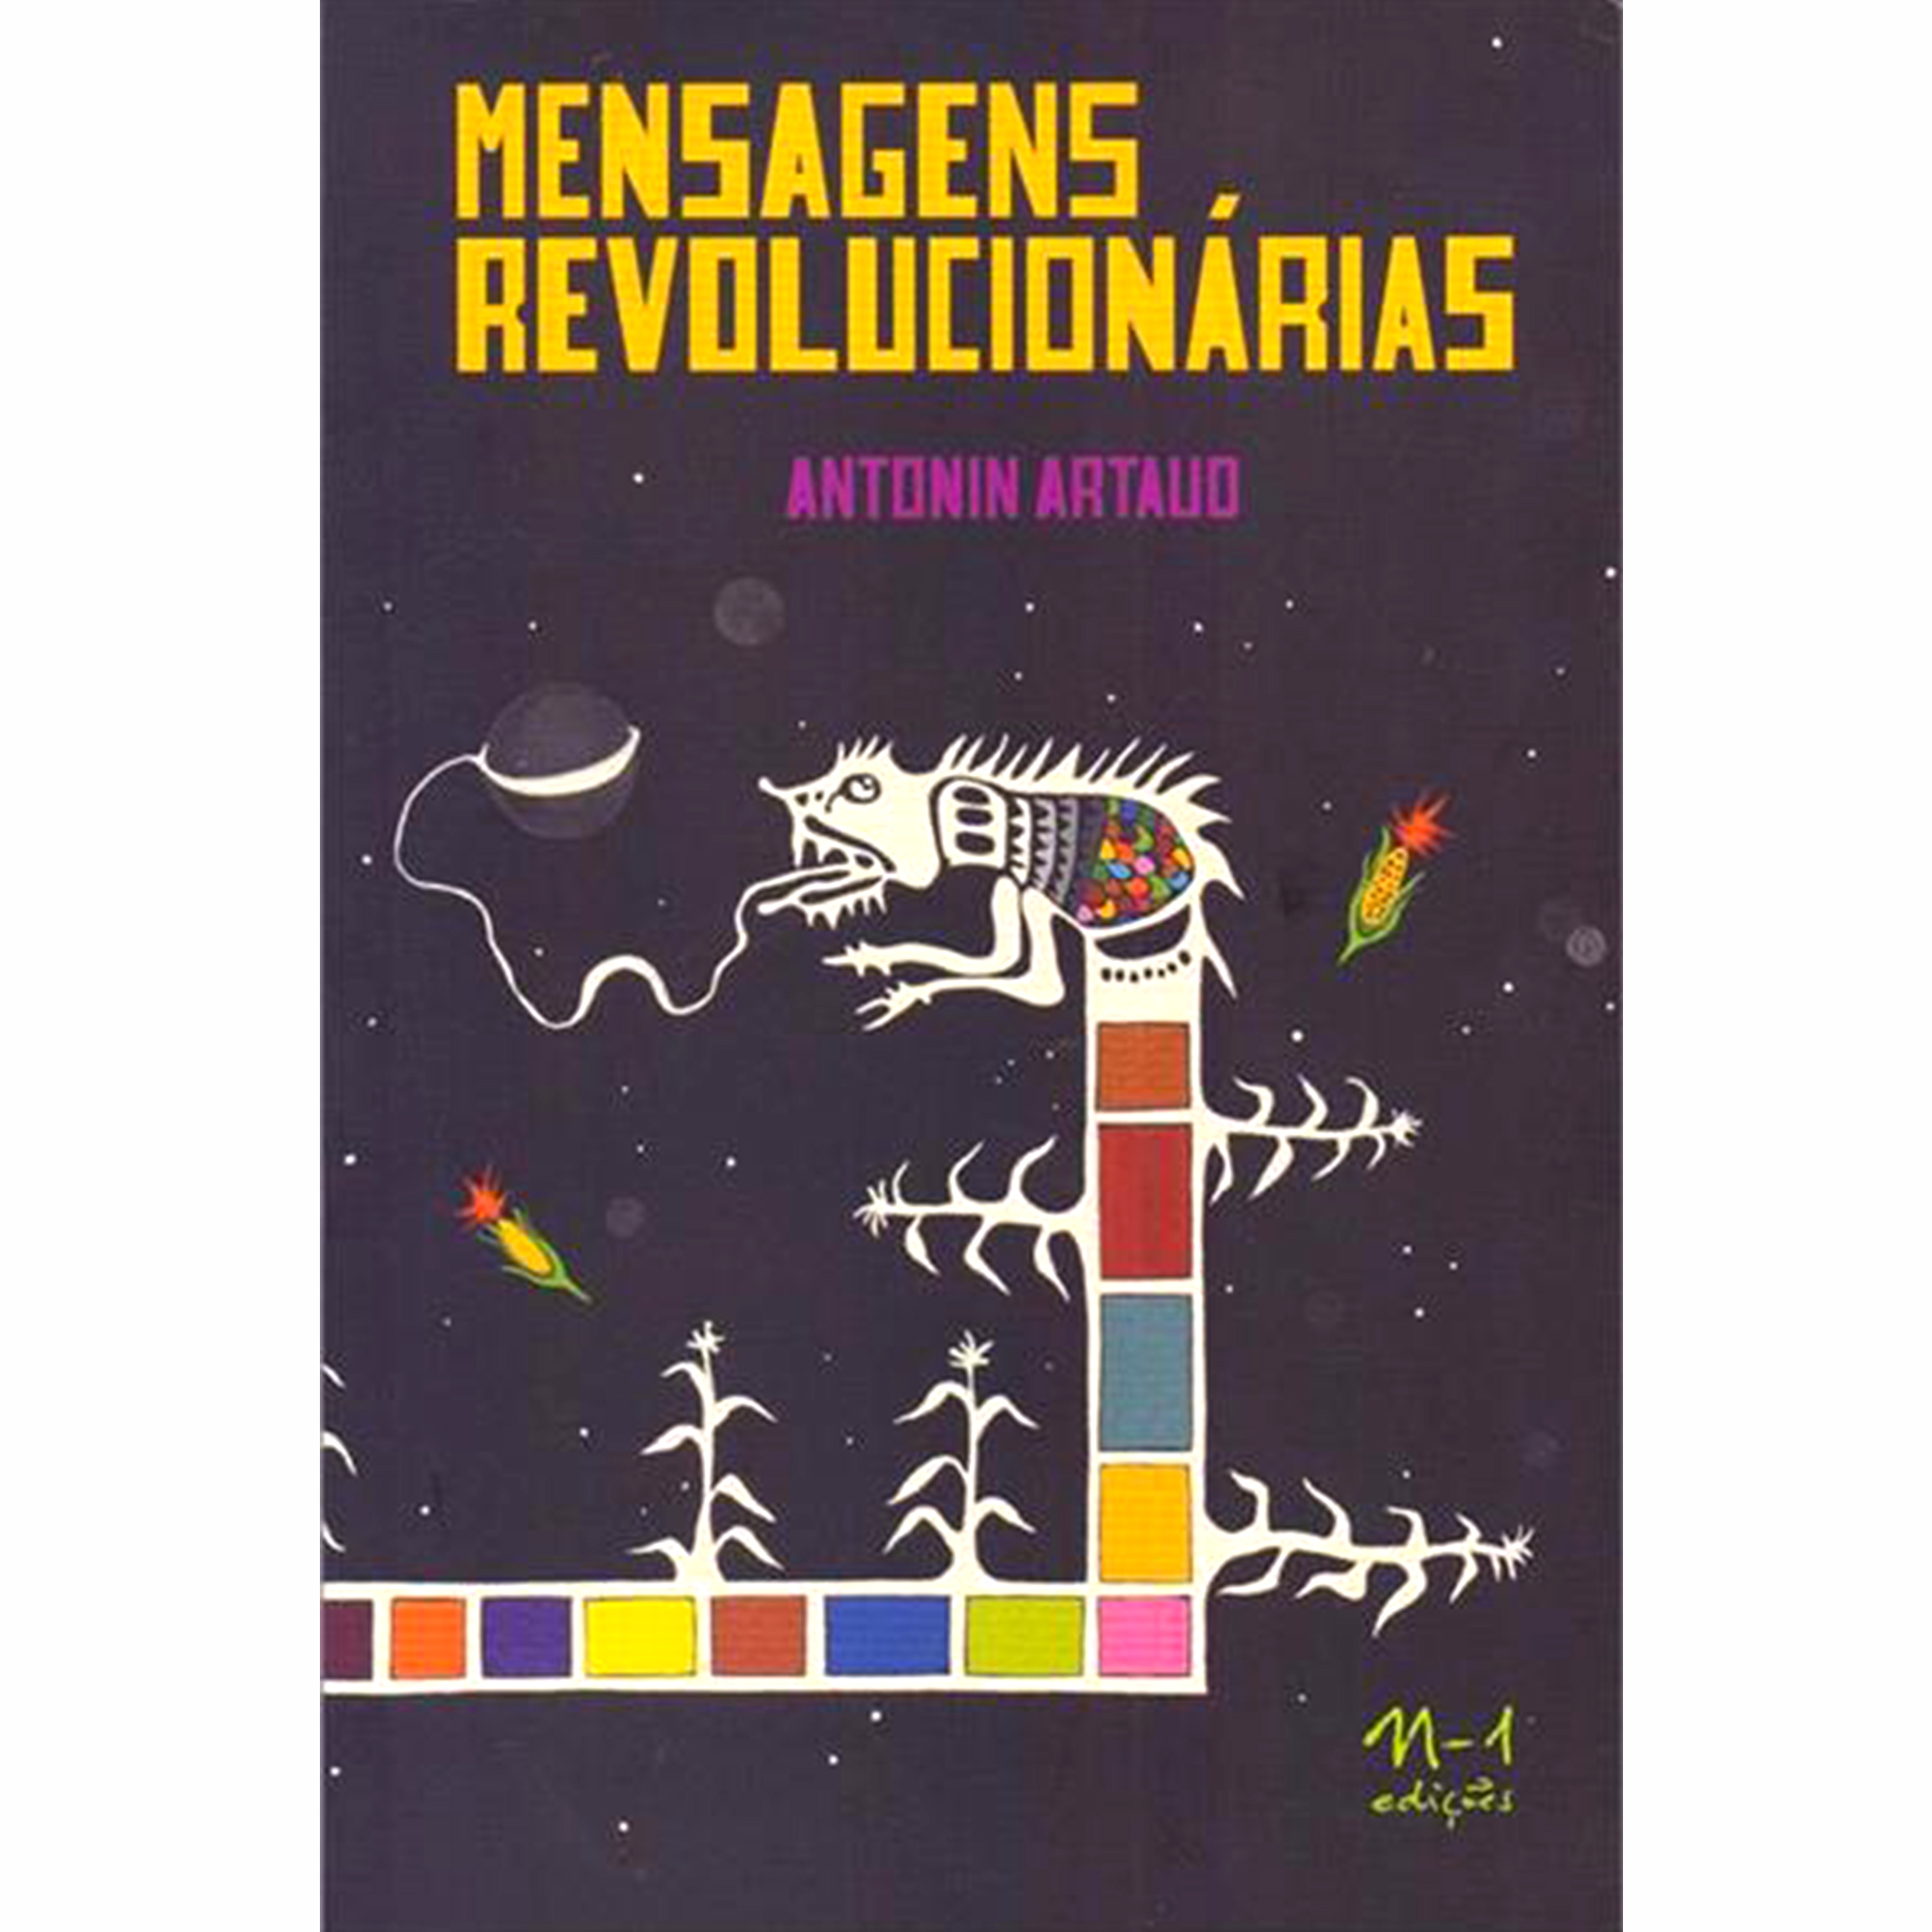
\includegraphics[width=74mm]{./CAPAS/mensagens.jpg}
\end{center}

\hspace*{-7cm}\hrulefill\hspace*{-7cm}

\medskip

\noindent{}Os textos, conferências e artigos aqui reunidos são fruto da estadia de Antonin Artaud no México, ocorrida em 1936. Mas afinal, o que Artaud foi fazer no México? É esta pergunta que acompanha a mente de quem percorre esses \textit{manifestos} sulfurosos. Eis a resposta do autor: \hlc{``Junto à revolução social e econômica indispensável, esperamos todos uma revolução da consciência que nos permitirá curar a vida. Cabe ao México moderno empreender essa revolução} (...) Nós esperamos do México, em suma, um novo conceito de revolução (...) e também um novo conceito do Homem''. Nesta frase encontramos a semente que nos inspira a avizinhar textos deixados por Artaud ao Movimento Zapatista.

\vfill

\hspace*{-.4cm}\begin{minipage}[c]{.5\linewidth}
\small\textbf{
\hspace*{-.1cm}Editora: n-1\\
Título: Mensagens revolucionárias\\
Autor: Antonin Artaud\\ 
ISBN: 978-65-86941-53-1\\
Páginas: 112\\
Formato: 14x21cm\\
Preço: R\$ 60,00\\
}
\end{minipage}

\pagebreak

\begin{center}
\hspace*{.5cm}
\includegraphics[width=74mm]{./CAPAS/animais.jpg}
\end{center}

\hspace*{-7cm}\hrulefill\hspace*{-7cm}

\medskip

\noindent{} Em \textit{O que os animais nos ensinam sobre política}, \hlc{o filósofo canadense Brian Massumi discute a questão do animal sob uma ótica inusitada. Noções tais como jogo, simpatia e criatividade, menosprezadas pela biologia evolucionista}, pelas ciências do comportamento animal ou pela filosofia, aqui são diretamente incorporadas ao conceito de natureza.

\vfill

\hspace*{-.4cm}\begin{minipage}[c]{.5\linewidth}
\small\textbf{
\hspace*{-.1cm}Editora: n-1\\
Título: O que os animais nos ensinam sobre política\\
Autor: Brian Mussumi\\
ISBN: 978-85-66943-47-4\\
Páginas: 192\\
Formato: 14x21\,cm\\
Preço: R\$ 55,00\\
}
\end{minipage}

\pagebreak

\begin{center}
\hspace*{-3.6cm}\raisebox{5cm}{\rotatebox[origin=t]{90}{\huge\textbf{Lançamento}}}
\hspace*{3.1cm}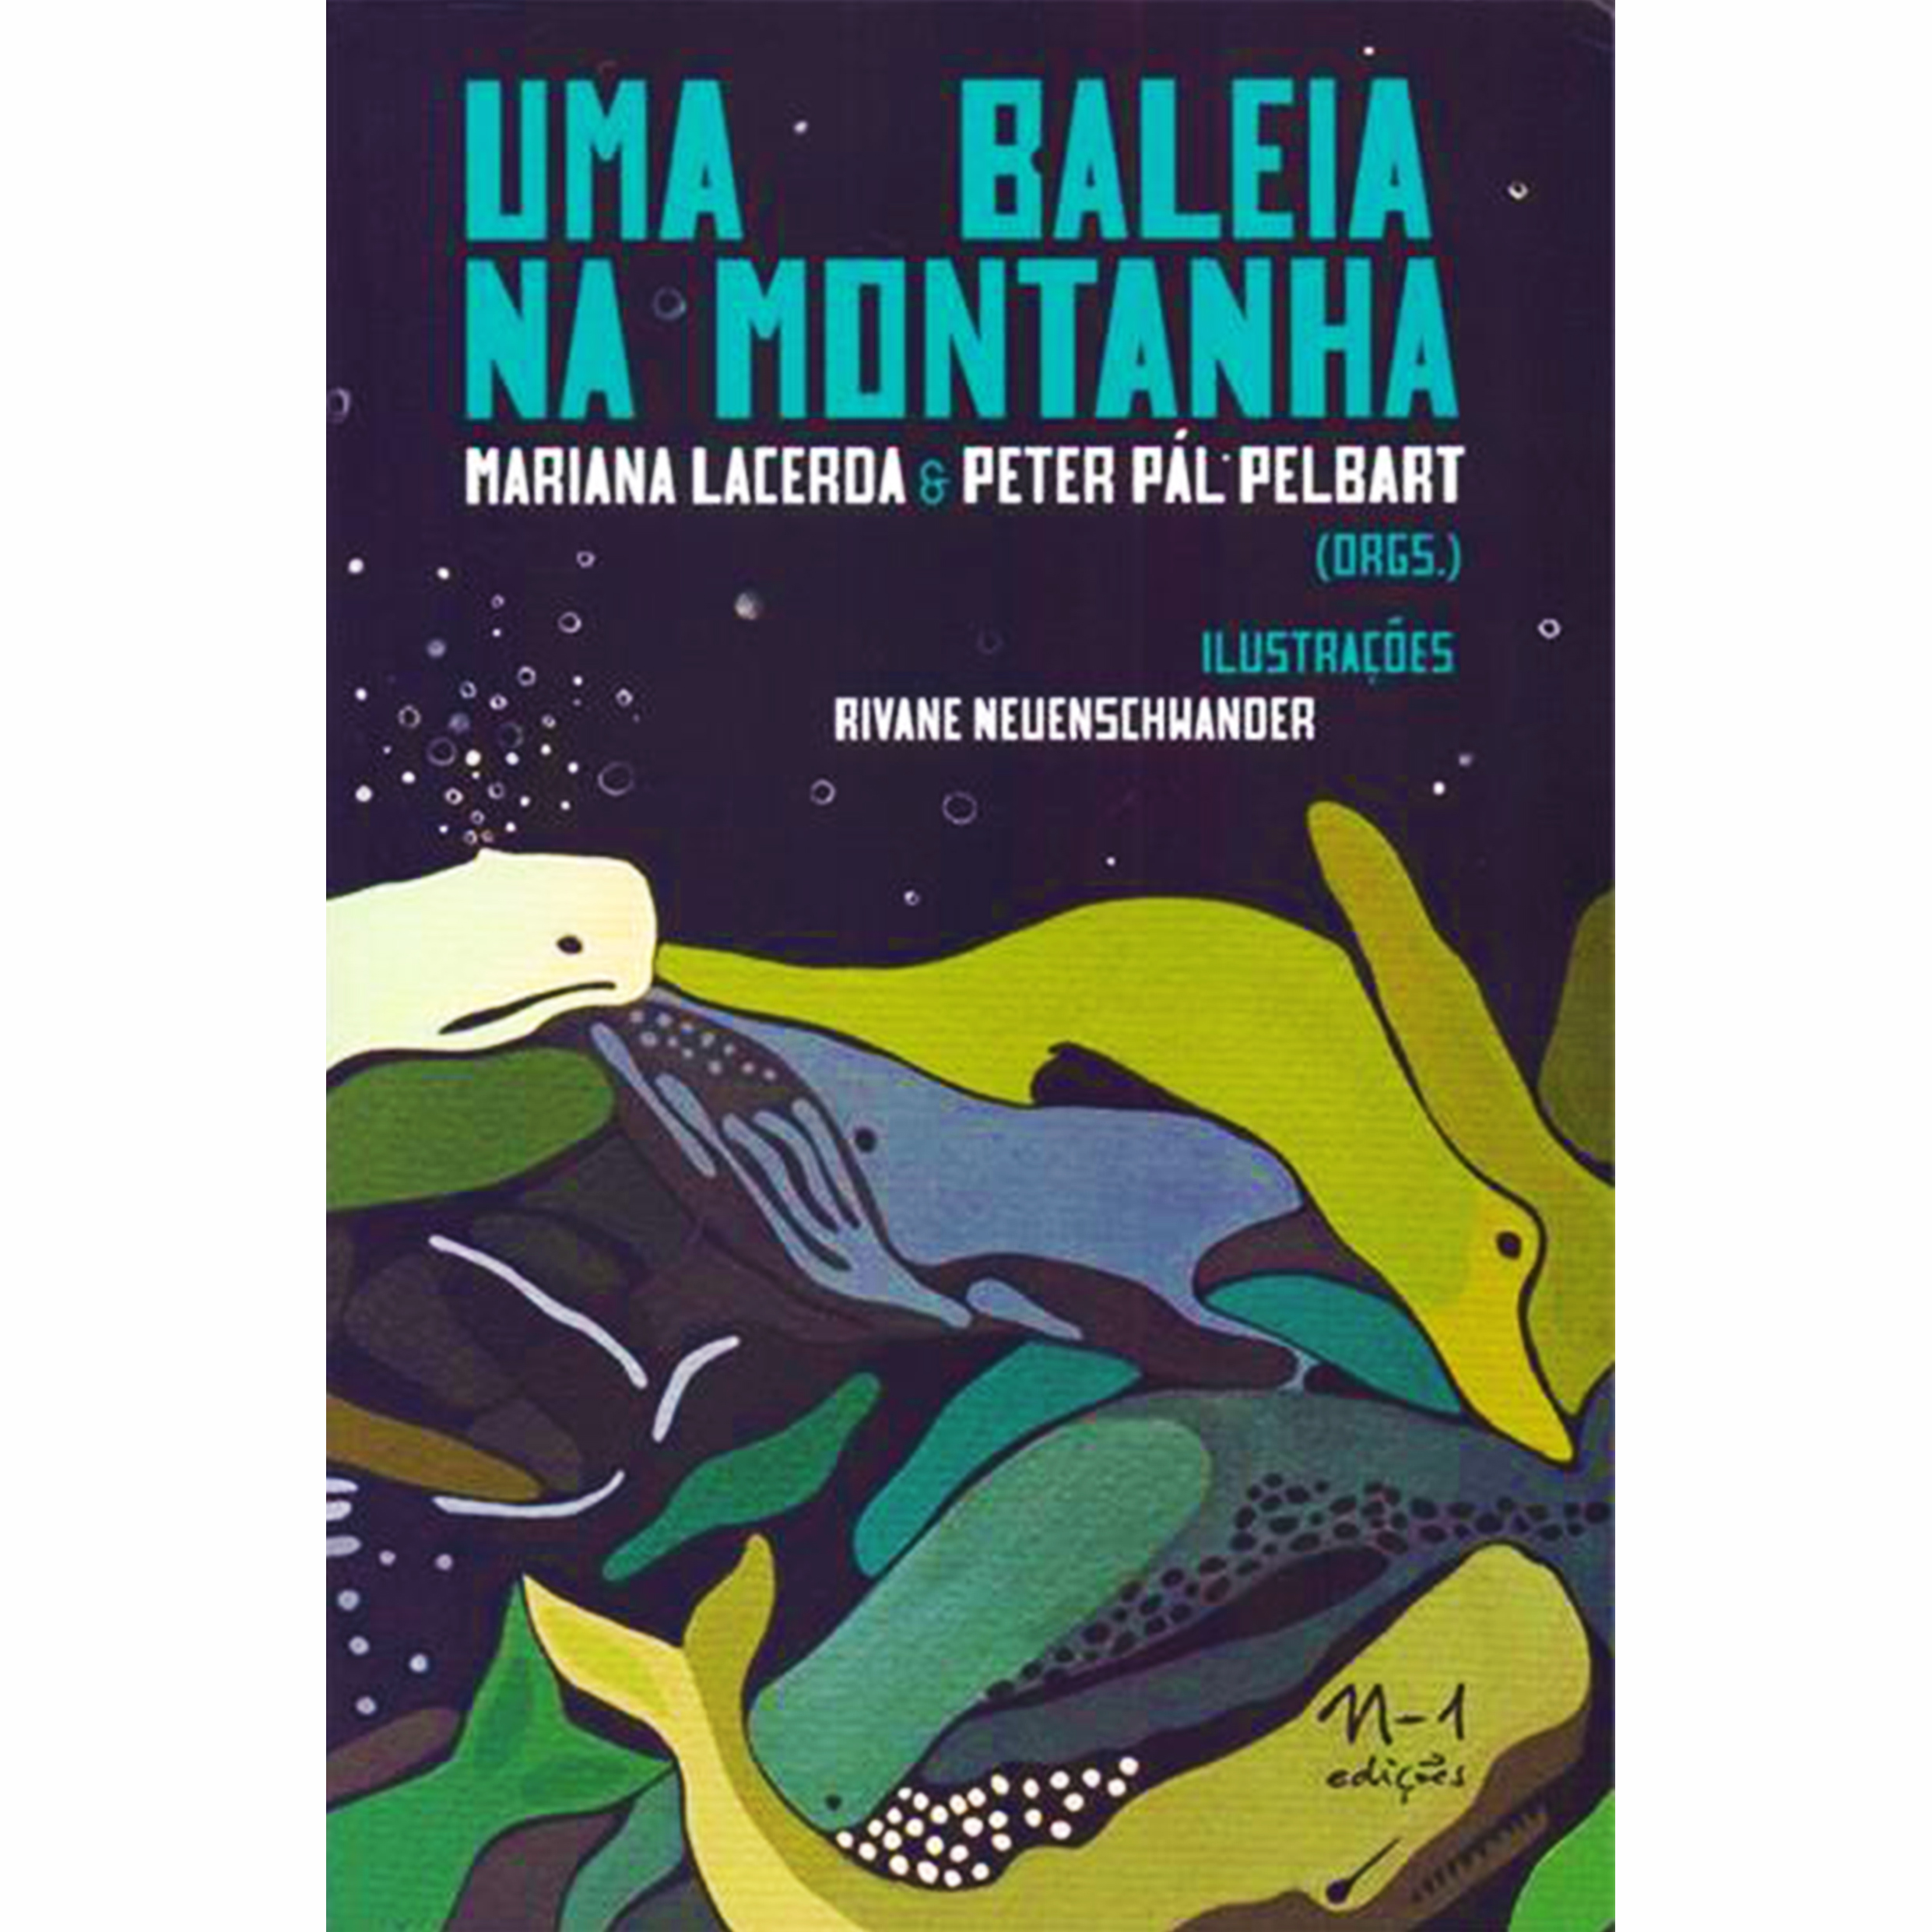
\includegraphics[width=74mm]{./CAPAS/baleia.jpg}
\end{center}

\hspace*{-7cm}\hrulefill\hspace*{-7cm}

\medskip

\noindent{}Para além de certos clichês, \hlc{pouco se sabe sobre o zapatismo no Brasil. Um movimento que parece ter surgido do nada, e às portas do terceiro milênio pega em armas, não para ensejar a militarização da luta, mas ao contrário, para chegar ao ponto em que se possa prescindir delas}. Um movimento que desmonetariza as trocas, rejeita a subserviência ao Estado e ao Capital, e a partir da herança maia reinventa as práticas comuns e as faz colocando a natureza, as mulheres, gays, trans e crianças no centro de seu mundo, sustentando o que os gregos chamavam de parrhesia, a palavra franca, o dizer-verdadeiro; para os maia: a \textit{palavra-espelho}. Um conto infantil do Subcomandante Marcos, com pinturas de Rivane Neuenschwander, é um convite especial às nossas crianças cujas almas parecem tão cansadas de telas.

\vfill

\hspace*{-.4cm}\begin{minipage}[c]{.5\linewidth}
\small\textbf{
\hspace*{-.1cm}Editora: n-1\\
Título: Uma baleia na montanha\\
Autor: Subcomandante Marcos\\ 
ISBN: 978-65-86941-32-6\\
Páginas: 288\\
Formato: 14x21cm\\
Preço: R\$ 87,00\\
}
\end{minipage}

\pagebreak

\begin{center}
\hspace*{.5cm}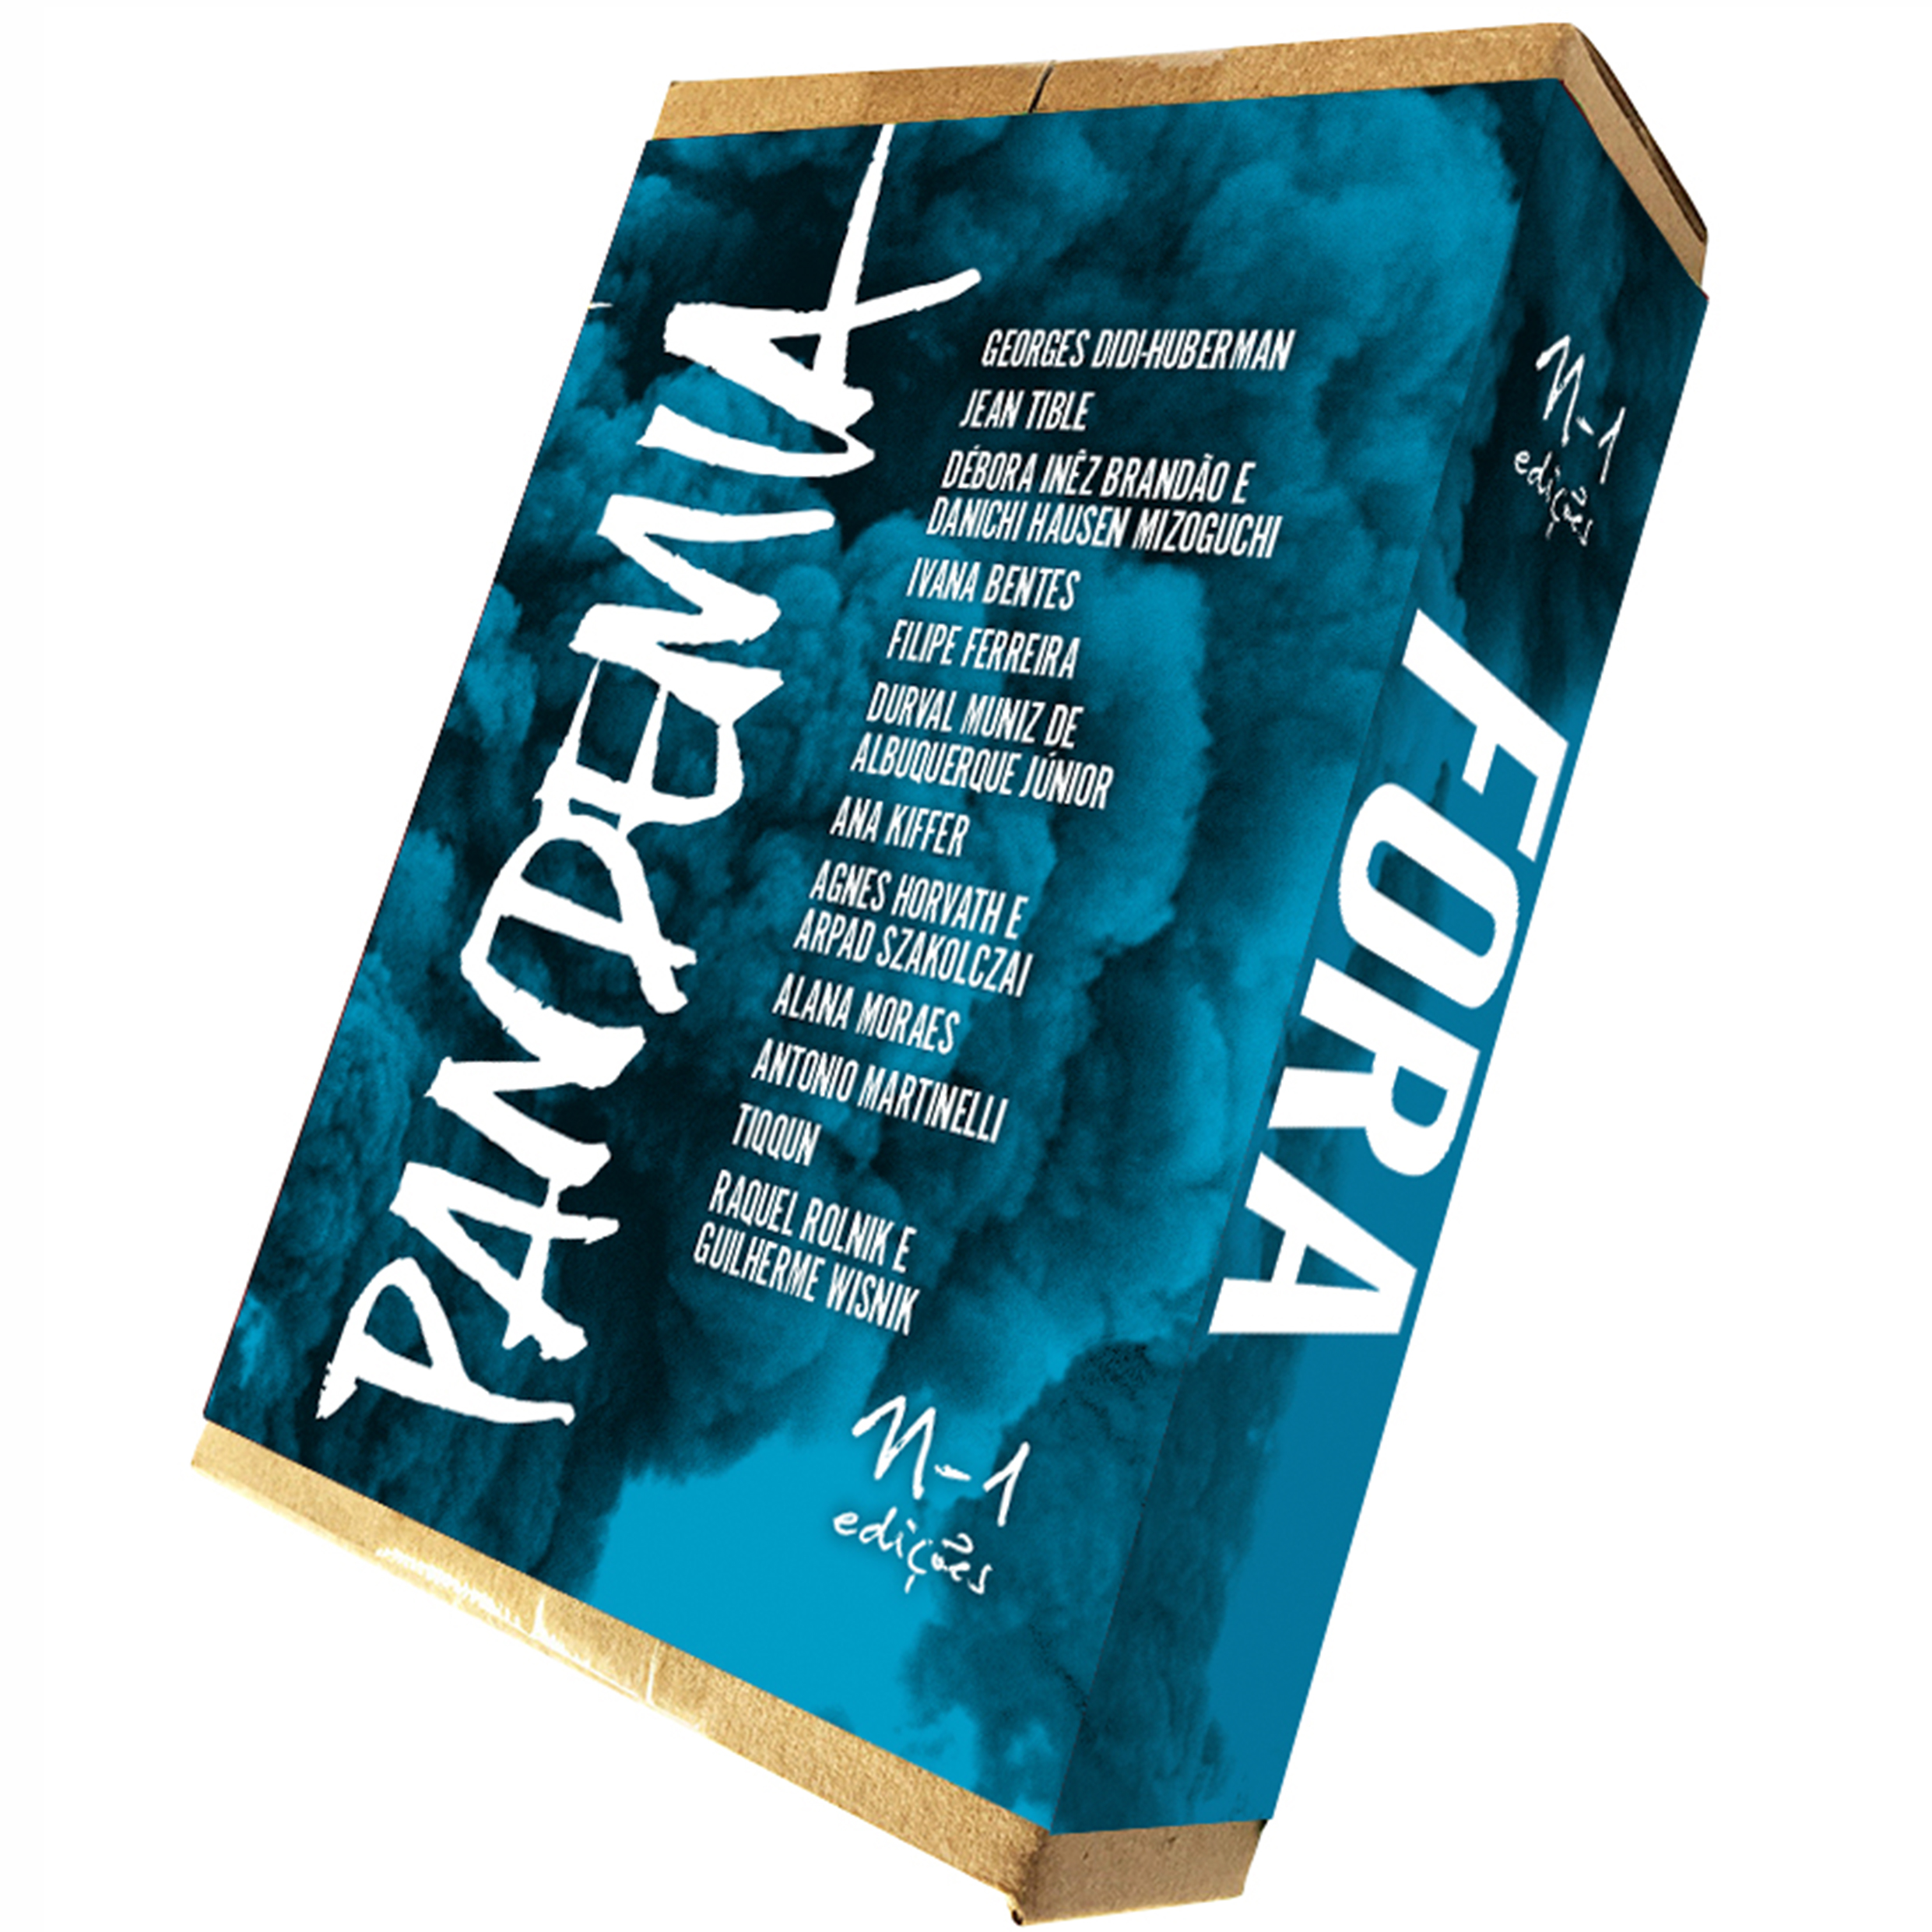
\includegraphics[width=74mm]{./CAPAS/caixa.jpg}
\end{center}

\hspace*{-7cm}\hrulefill\hspace*{-7cm}

\medskip

\noindent{} Caixa \hlc{composta por 12 textos dos seguintes autores}: Georges Didi-Huberman, Débora Inêz Brandão, Danich Hausen Mizoguchi, Durval Muniz de Albuquerque Júnior, Tiqqun, Ivana Bentes, Filipe Ferreira, Ana Kiffer, Agnes Horvath, Arpad Szakolczai, Alana Moraes, Antonio Martinelli, Jean Tible, Raquel Rolnik e Guilherme Wisnik.

\vfill

\hspace*{-.4cm}\begin{minipage}[c]{.5\linewidth}
\small\textbf{
\hspace*{-.1cm}Editora: n-1\\
Título: Caixa Fora\\
Autor: Vários\\
ISBN: 978-65-86941-48-7\\
Páginas: 355\\
Formato: 19x11\,cm\\
Preço: R\$ 85,00\\
}
\end{minipage}

\pagebreak

\begin{center}
\hspace*{.5cm}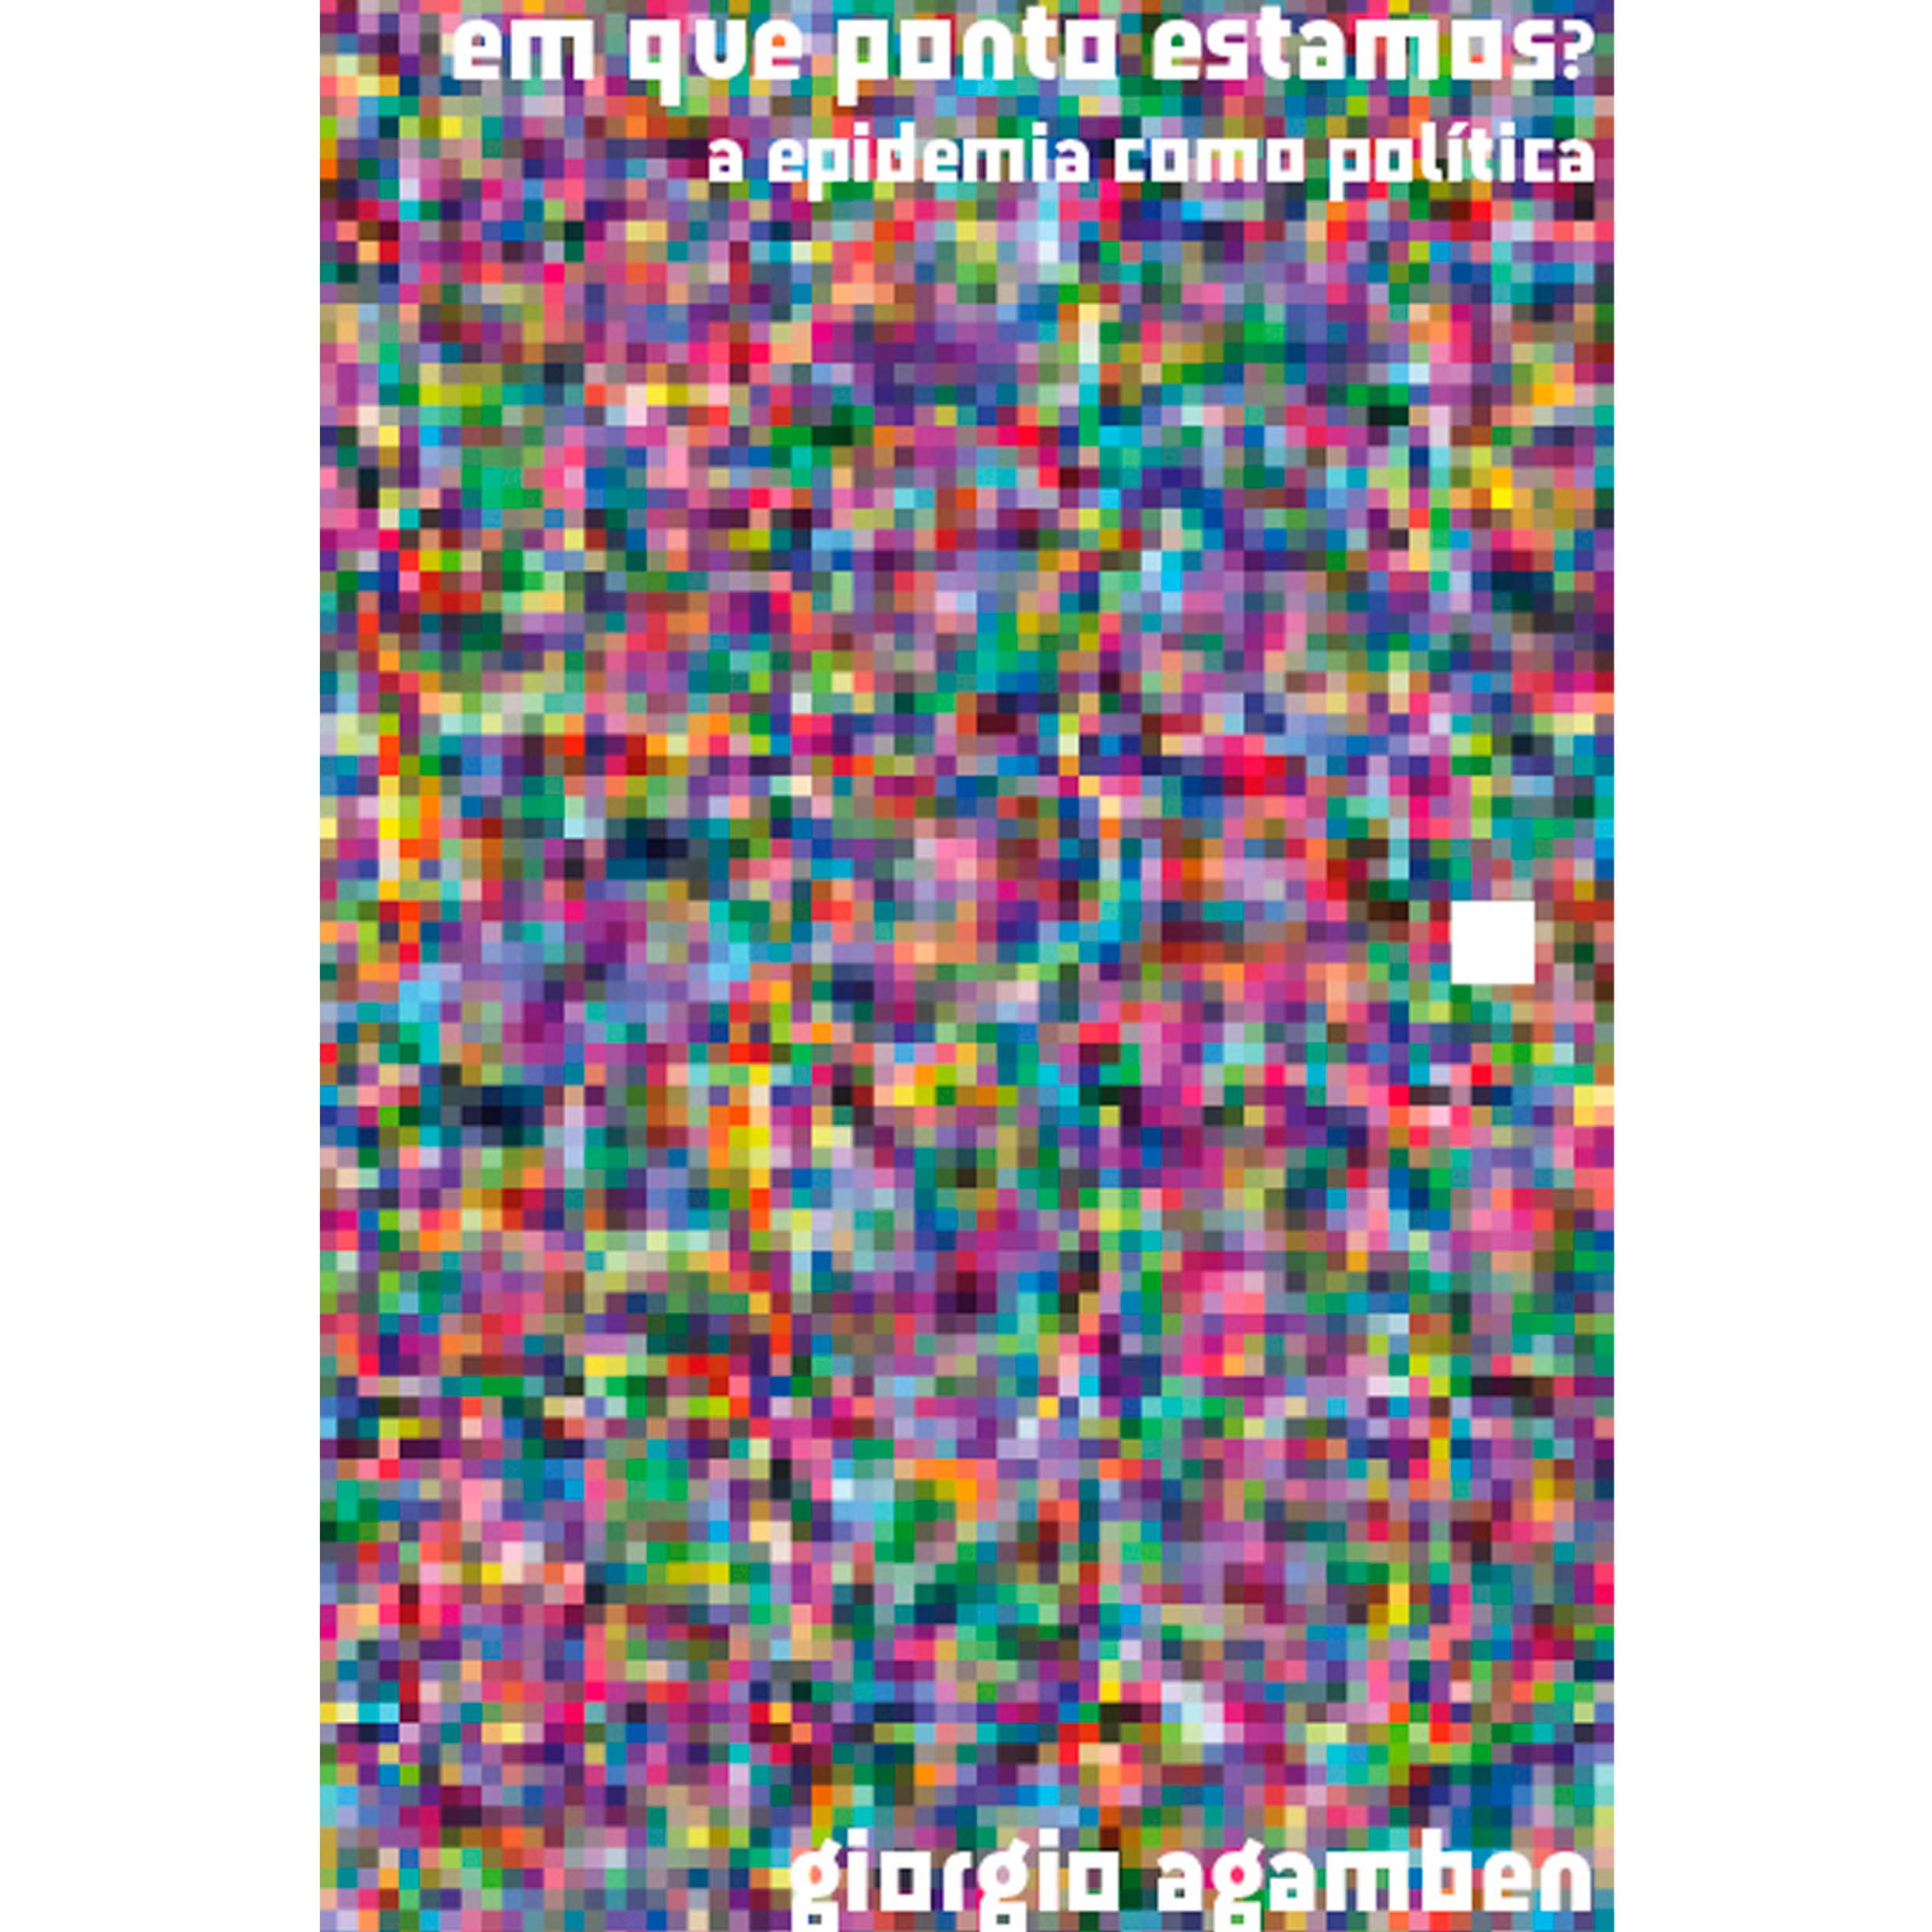
\includegraphics[width=74mm]{./CAPAS/agamben.jpg}
\end{center}

\hspace*{-7cm}\hrulefill\hspace*{-7cm}

\medskip

\noindent{}(...)Teremos, em uma palavra, que nos colocar seriamente a única pergunta que conta, que não é, como repetem há séculos os falsos filósofos, ``de onde viemos'' ou ``para onde vamos?'', mas, simplesmente, ``em que ponto estamos?''. Esta é a pergunta à qual deveremos tentar responder, do modo que pudermos e onde quer que estejamos, mas, em todo caso, com a nossa vida e não apenas com as palavras.(...)

\vfill

\hspace*{-.4cm}\begin{minipage}[c]{1\linewidth}
\small\textbf{
\hspace*{-.1cm}Editora: n-1\\
Título: Em que ponto estamos?\\
Autor: Giorgio Agamben\\
ISBN: 978-65-86941-55-5\\
Páginas: 128\\
Formato: 21x14\,cm\\
Preço: R\$ 68,00\\
}
\end{minipage}

\pagebreak


\begin{center}
\hspace*{.5cm}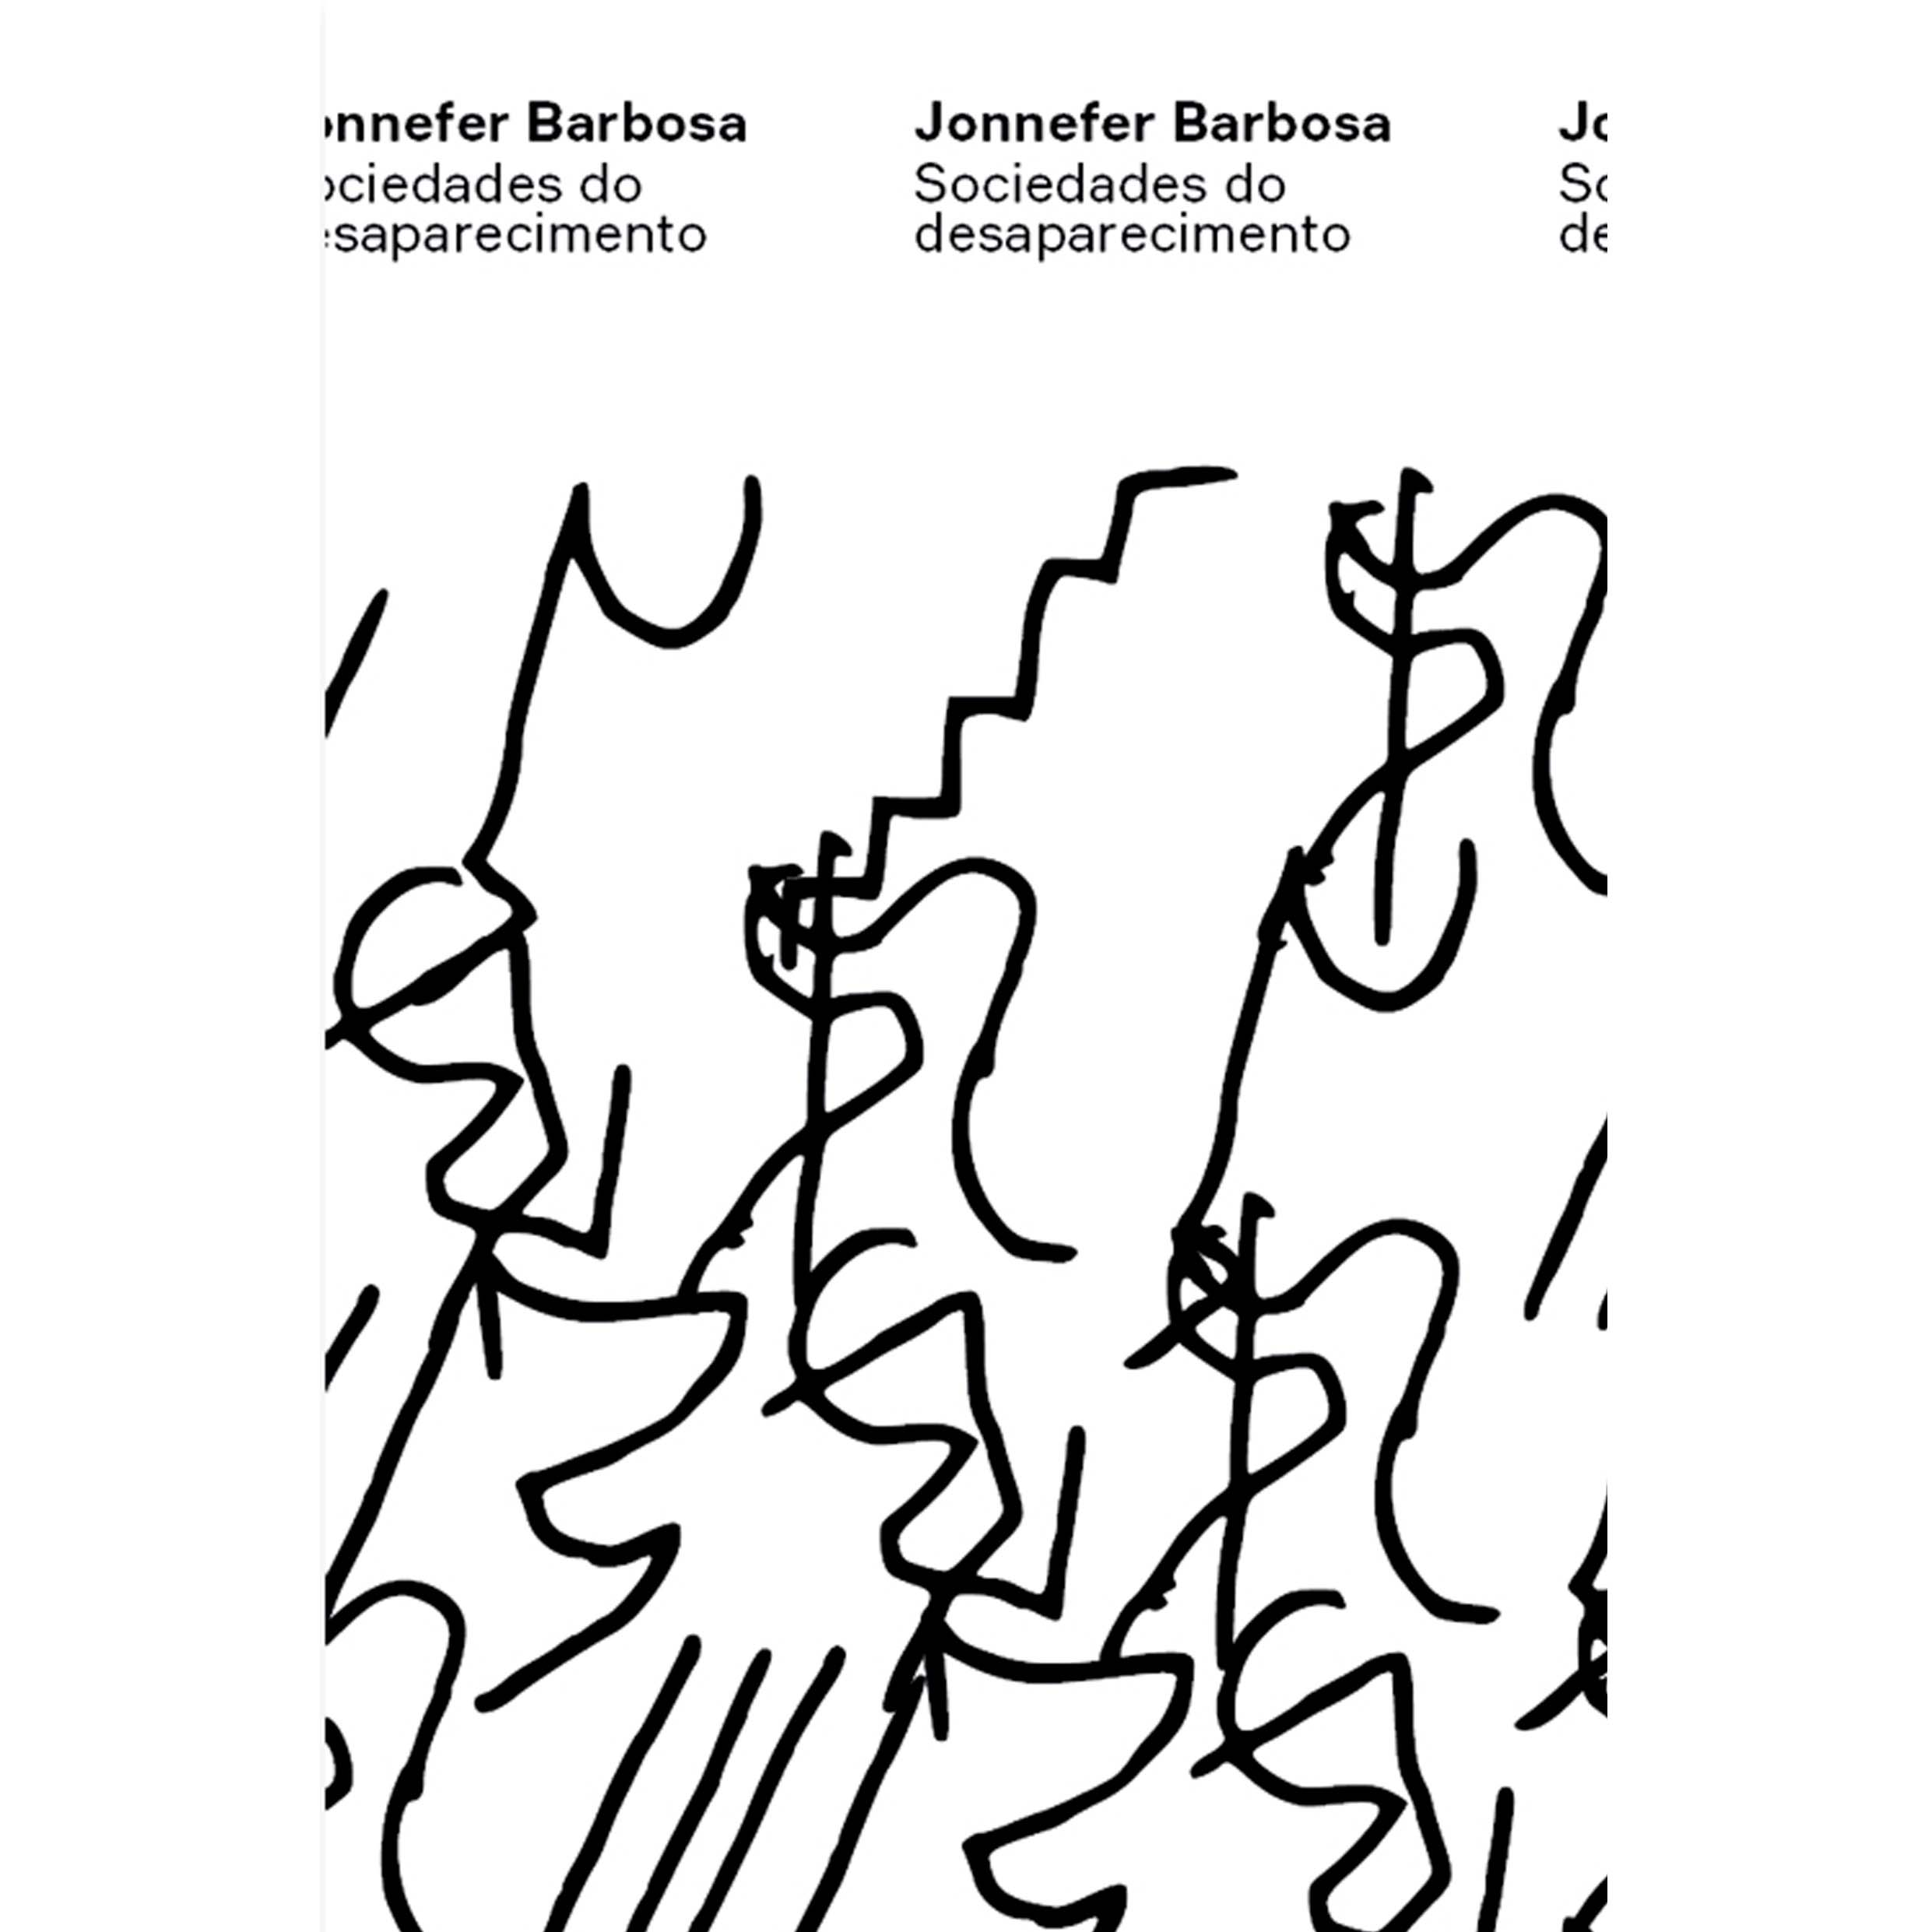
\includegraphics[width=74mm]{./CAPAS/barbosa.jpg}
\end{center}

\hspace*{-7cm}\hrulefill\hspace*{-7cm}

\medskip

\noindent{}

\vfill

\hspace*{-.4cm}\begin{minipage}[c]{1\linewidth}
\small\textbf{
\hspace*{-.1cm}Editora: n-1\\
Título: Sociedades do desaparecimento\\
Autor: Jonnefer Barbosa\\
ISBN: 978-65-86941-43-2\\
Páginas: 80\\
Formato: 18x11\,cm\\
Preço: R\$ 44,00\\
}
\end{minipage}

\pagebreak

\begin{center}
\hspace*{.5cm}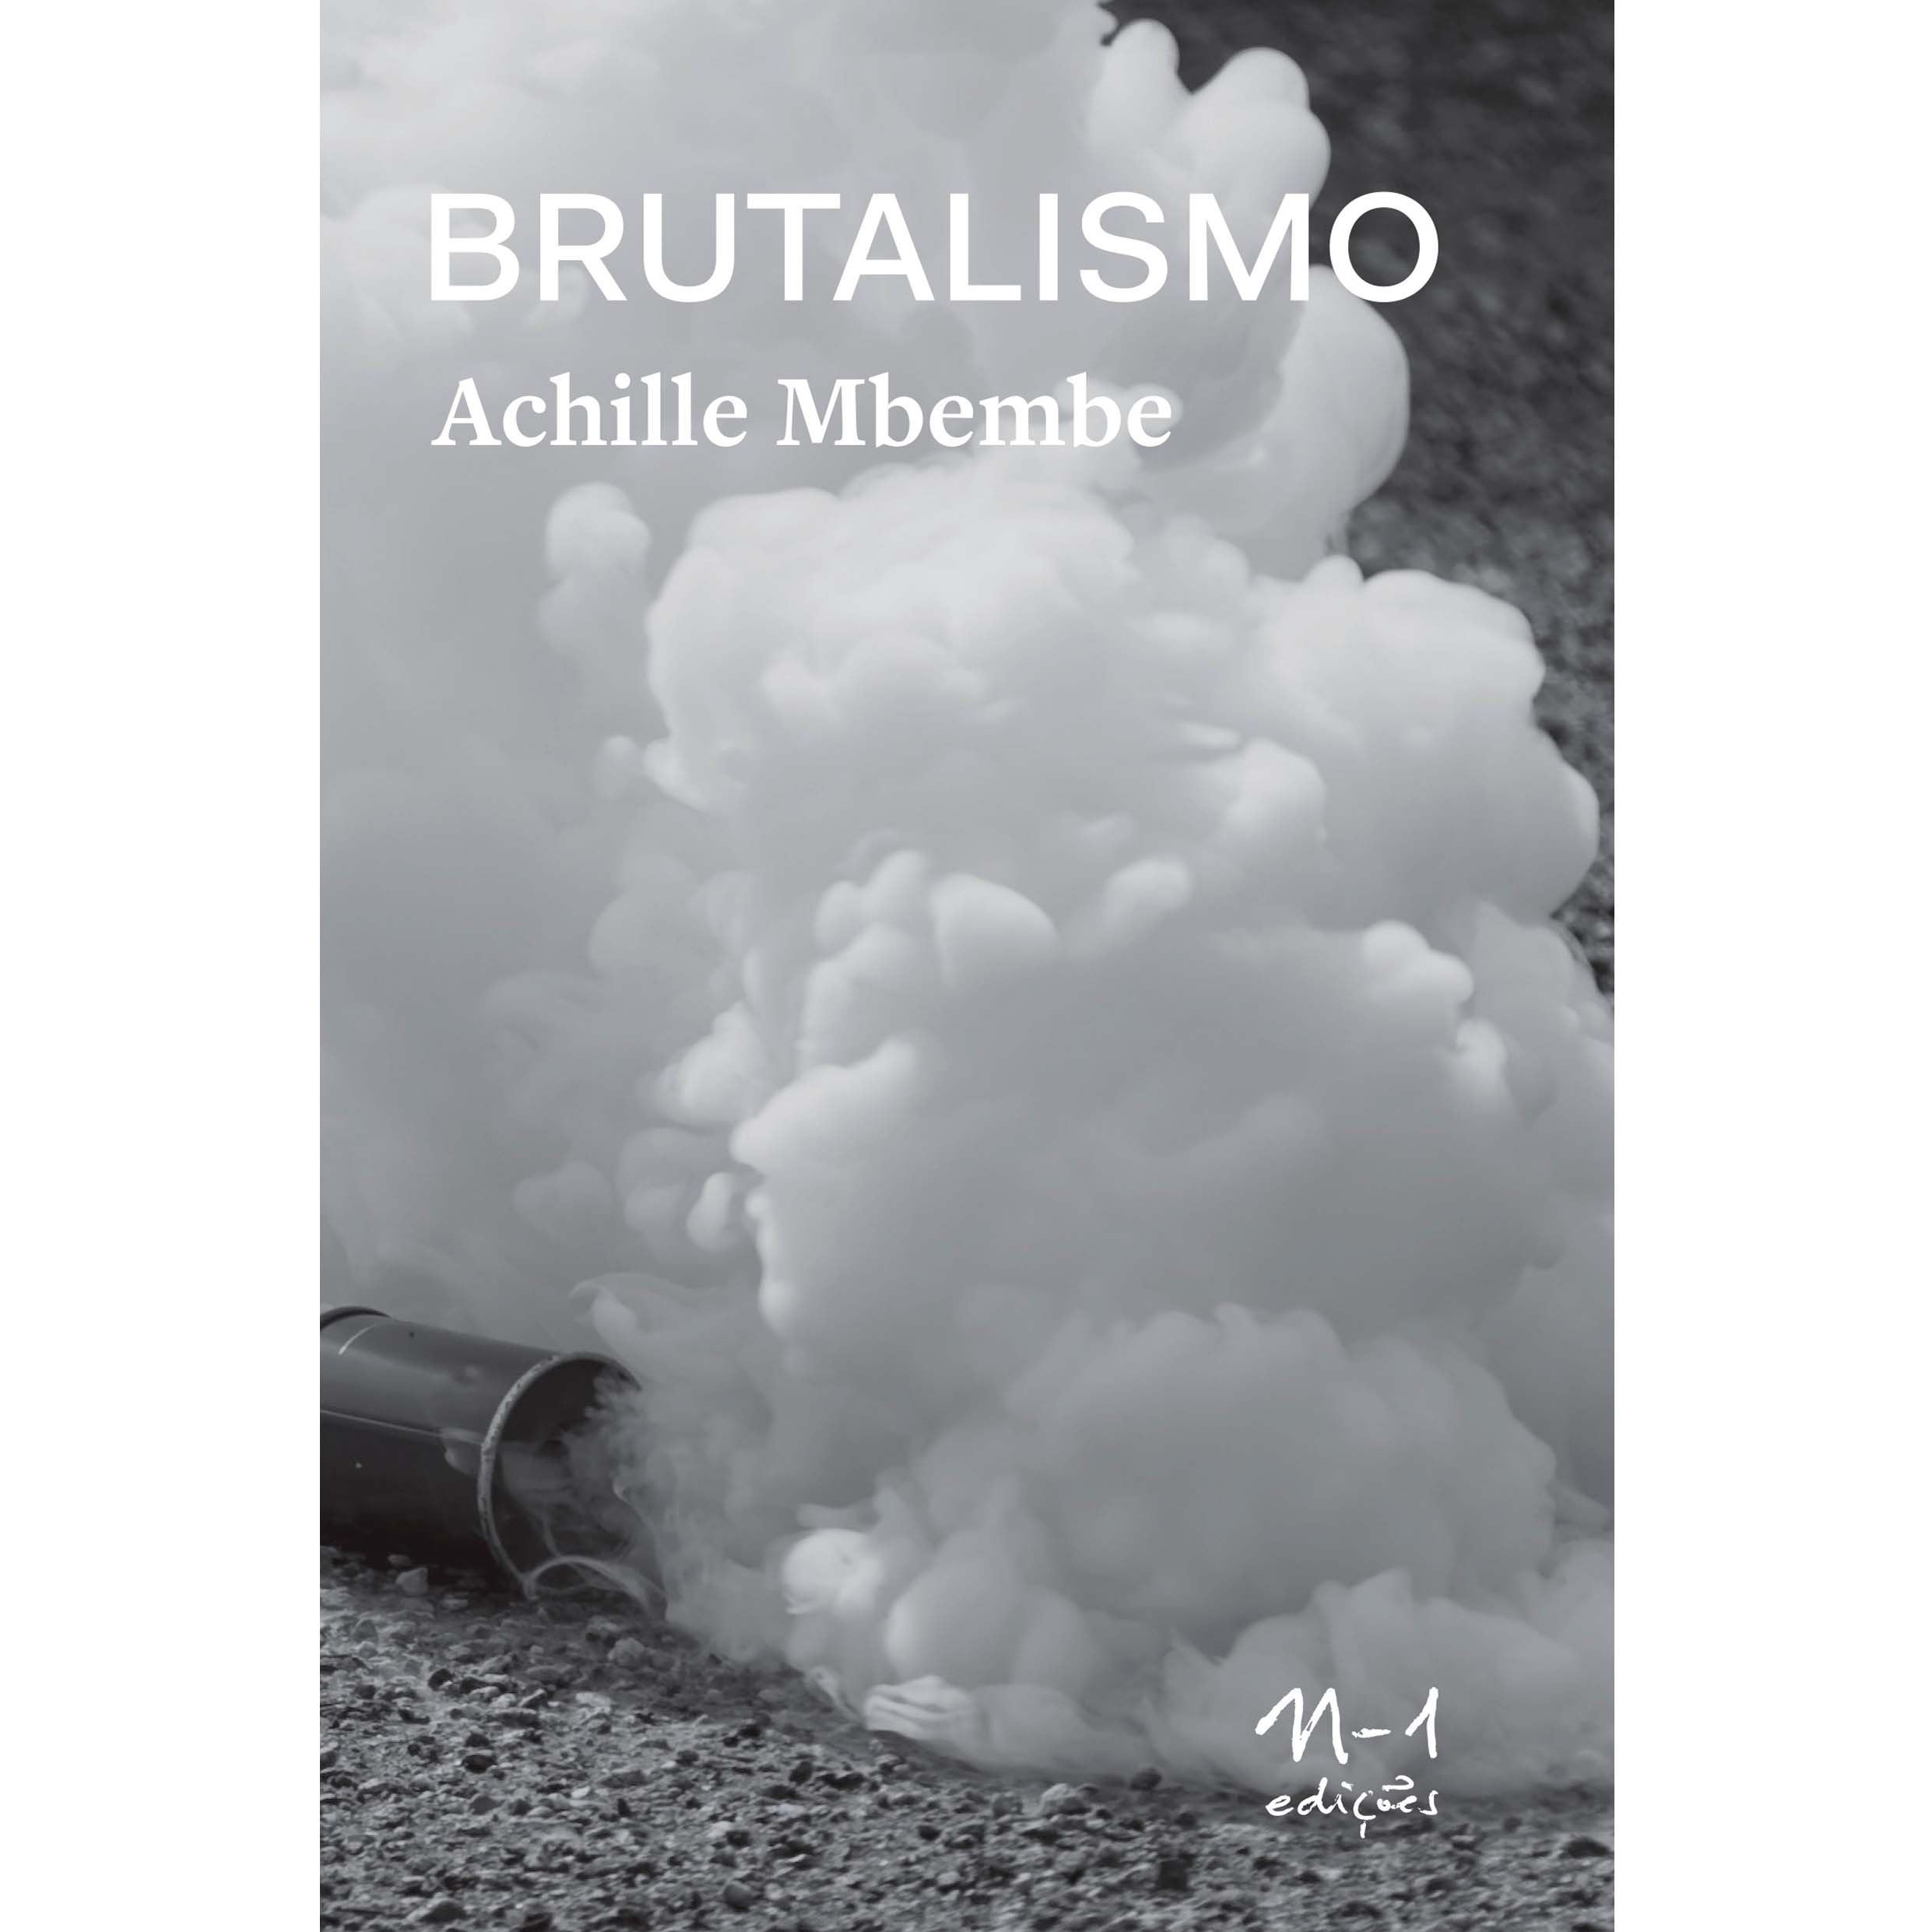
\includegraphics[width=74mm]{./CAPAS/brutalismo.jpg}
\end{center}

\hspace*{-7cm}\hrulefill\hspace*{-7cm}

\medskip

\noindent{}(...)Um vasto empreendimento de ocupação territorial, de domínio sobre os corpos e os imaginários, de desmontagem, dissociação e demolição está em curso. Ele conduz, praticamente em toda parte, a ``estados de emergência'' ou ``estados de exceção'', que logo se estendem e se tornam permanentes. As modalidades contemporâneas de demolição se cristalizam, enquanto as clássicas dicotomias forma/matéria, matéria/material, material/imaterial, natural/artificial e fim/meio são profundamente questionadas. A lógica das oposições foi substituída pela das permutações, convergências e conversões múltiplas. Não há mais nenhuma matéria intrinsecamente disponível e dócil. Ela existe apenas coconstituída a partir de uma heterogeneidade de matrizes e conexões.(...)

\vfill

\hspace*{-.4cm}\begin{minipage}[c]{1\linewidth}
\small\textbf{
\hspace*{-.1cm}Editora: n-1\\
Título: Brutalismo\\
Autor: Achille Mbembe\\
ISBN: 978-65-86941-62-3\\
Páginas: 256\\
Formato: 21x14\,cm\\
Preço: R\$ 90,00\\
}
\end{minipage}

\pagebreak

\begin{center}
\hspace*{.5cm}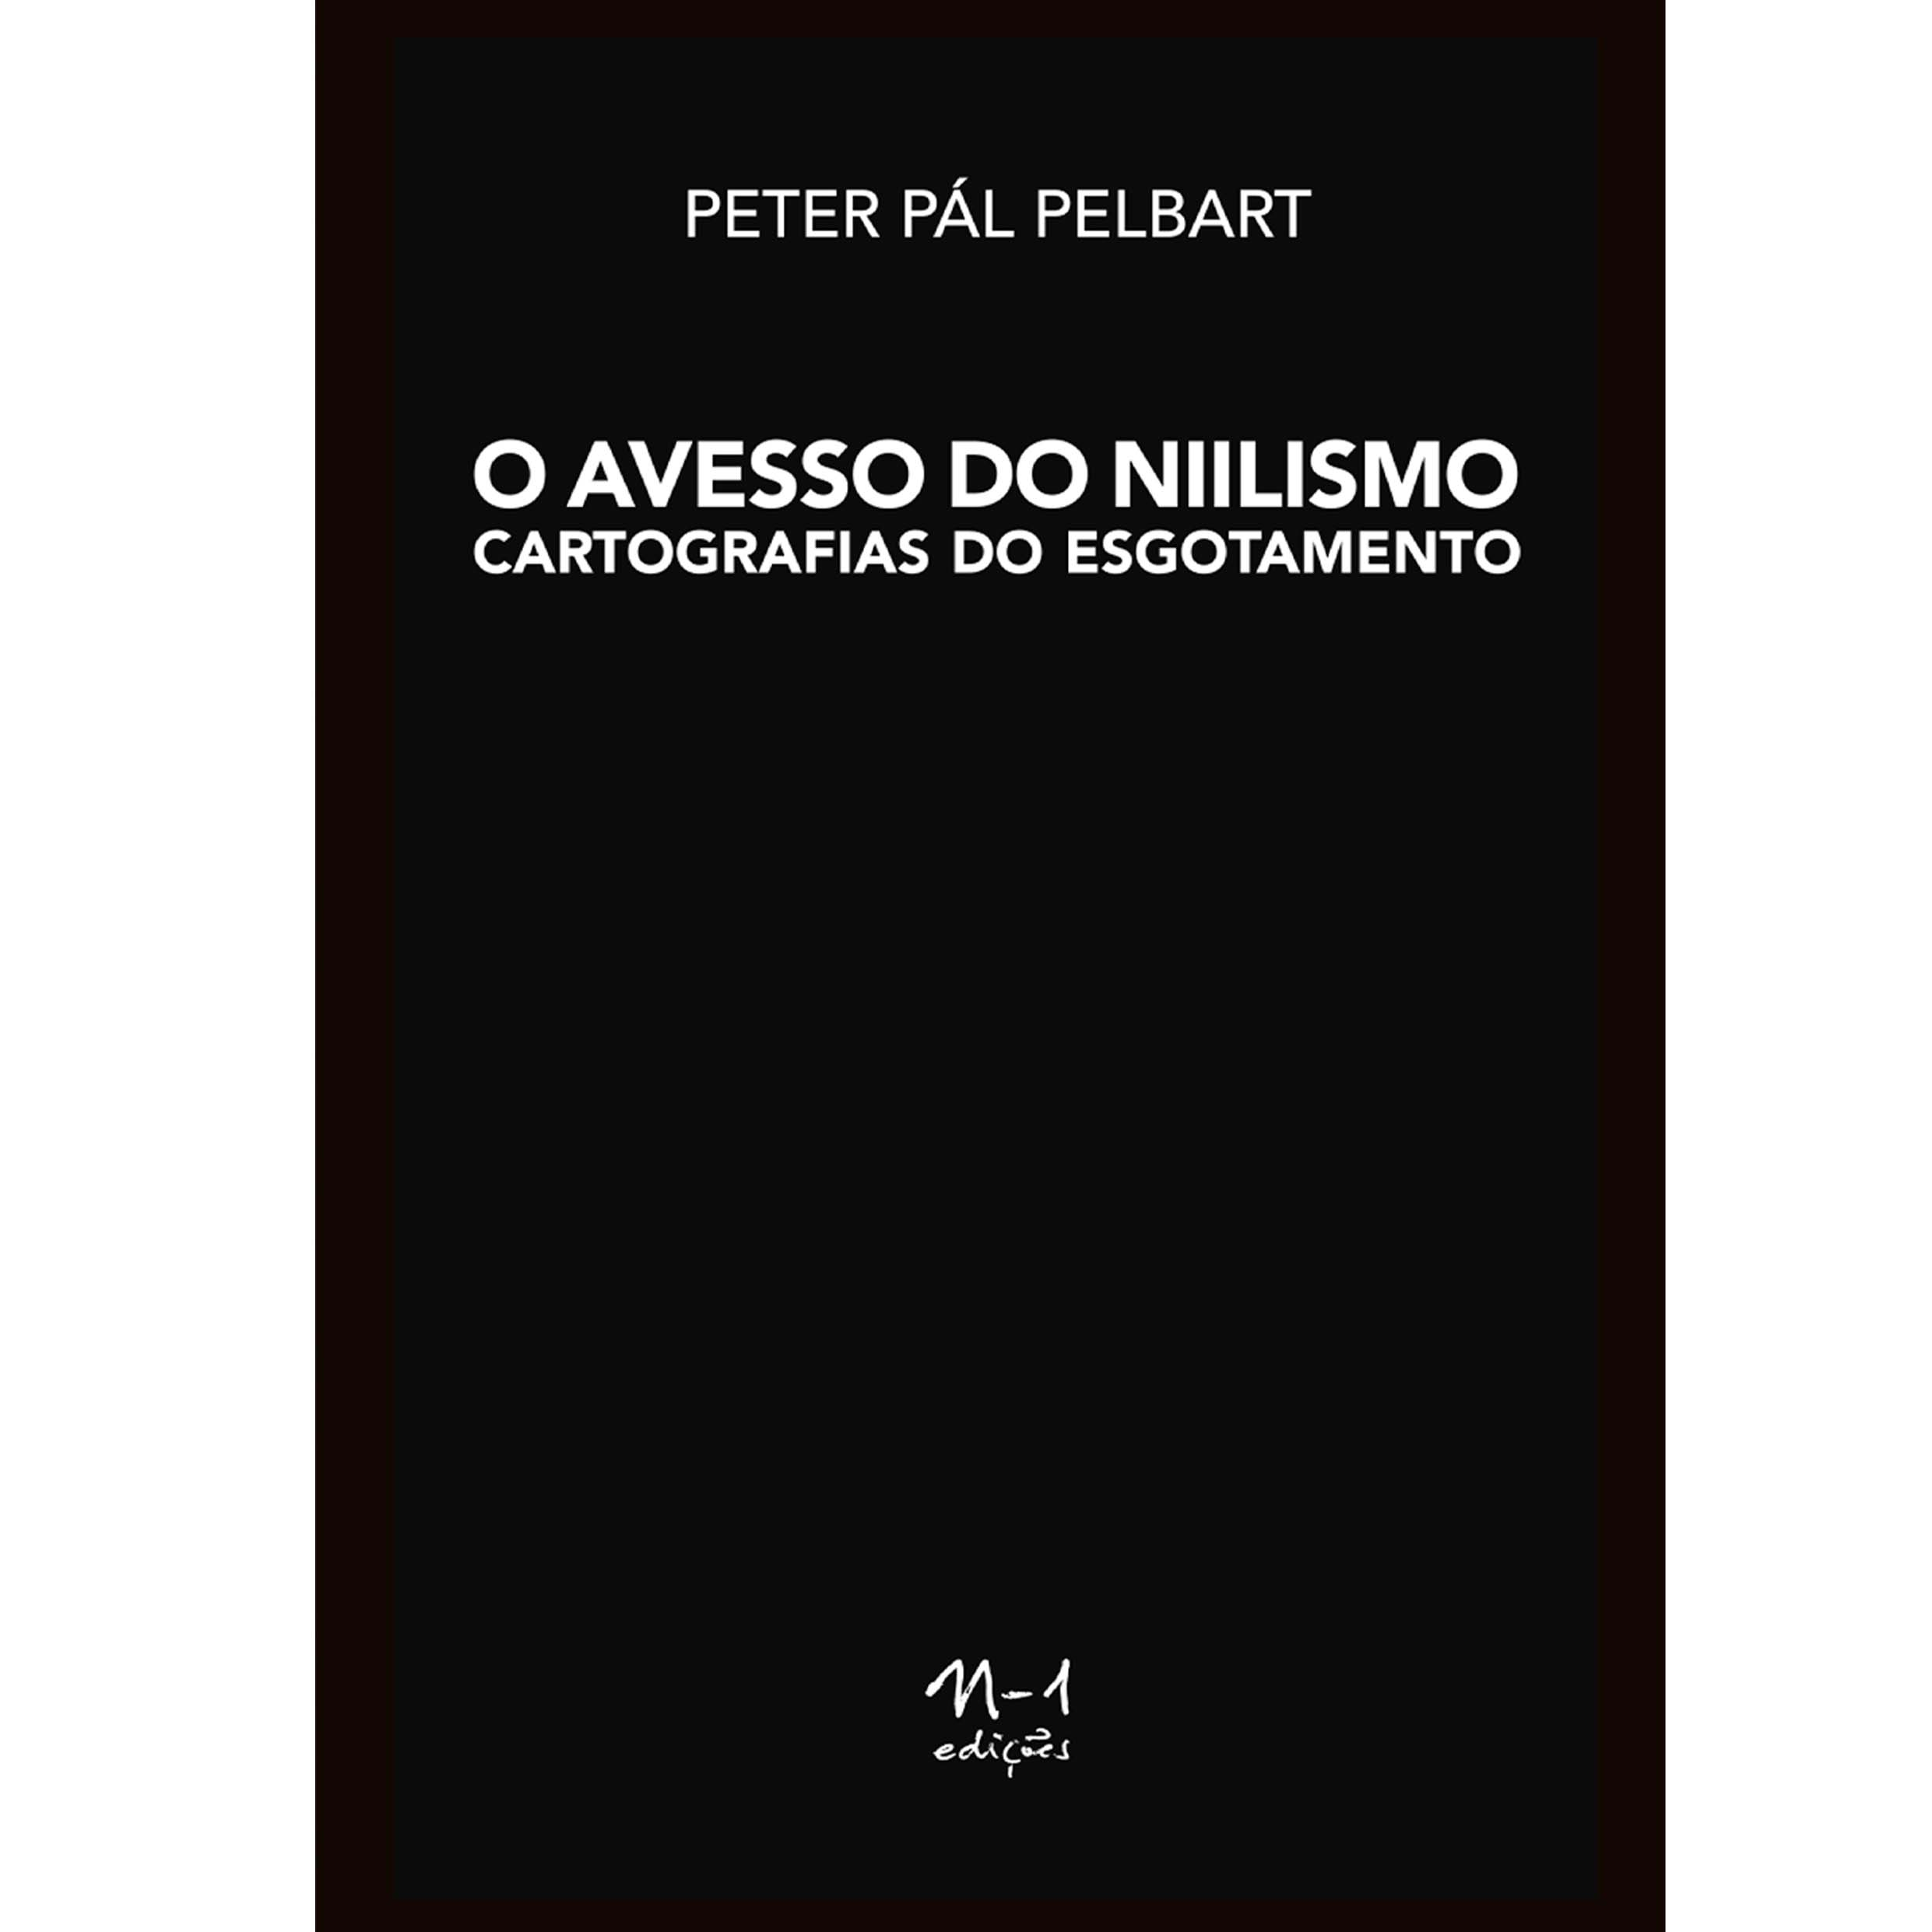
\includegraphics[width=74mm]{./CAPAS/pelbart.jpg}
\end{center}

\hspace*{-7cm}\hrulefill\hspace*{-7cm}

\medskip

\noindent{}Afinal, do que é que estamos tão esgotados, hoje? Inspirado em um vasto leque de autores, de Musil a Blanchot, de Deleuze a Agamben, de Jünger a Sloterdijk, mas também apoiado em experiências"-limite extraídas de Deligny ou de algum trabalho esquizo"-cênico, o livro que o leitor tem em mãos apresenta indícios, mesmo fugidios, de um deslocamento em curso. De quem? Do quê? Em qual direção? Não sabemos ao certo. É uma cartografia coletiva, inacabada, movente, que indica pontos de estrangulamento através dos quais, nos avessos do niilismo biopolítico, se liberam outras energias, visões, noções. Não se trata, portanto, de saber ``quem fala'', nem ``de qual lugar se fala'', talvez nem mesmo ``do que'' se fala, mas, como o sugeriu Guattari, ``o que fala através de nós''. É preciso imaginar uma cartografia do esgotamento que fosse uma espécie de sintomatologia molecular, como em Beckett. Ali, figuras extremas como esgotamento, desastre, catástrofe, e mesmo caosmose, tangenciam pontos de a"-fundamento onde aparecem, paradoxalmente e ao mesmo tempo, os contramovimentos do presente. É nesses pontos de inflexão que se insinuam, de maneira às vezes imperceptível, os contragolpes minúsculos, mas também as explosões multitudinárias que denunciam o que caducou (valores, estilos, problemas), ao mesmo tempo em que deixam entrever novos desejos e necessidades.

\vfill

\hspace*{-.4cm}\begin{minipage}[c]{1\linewidth}
\small\textbf{
\hspace*{-.1cm}Editora: n-1\\
Título: O avesso do niilismo\\
Autor: Peter Pál Pelbart\\
ISBN: 978-65-86941-64-7\\
Páginas: 448\\
Formato: 21x14\,cm\\
Preço: R\$ 68,00\\
}
\end{minipage}

\pagebreak

\begin{center}
\hspace*{.5cm}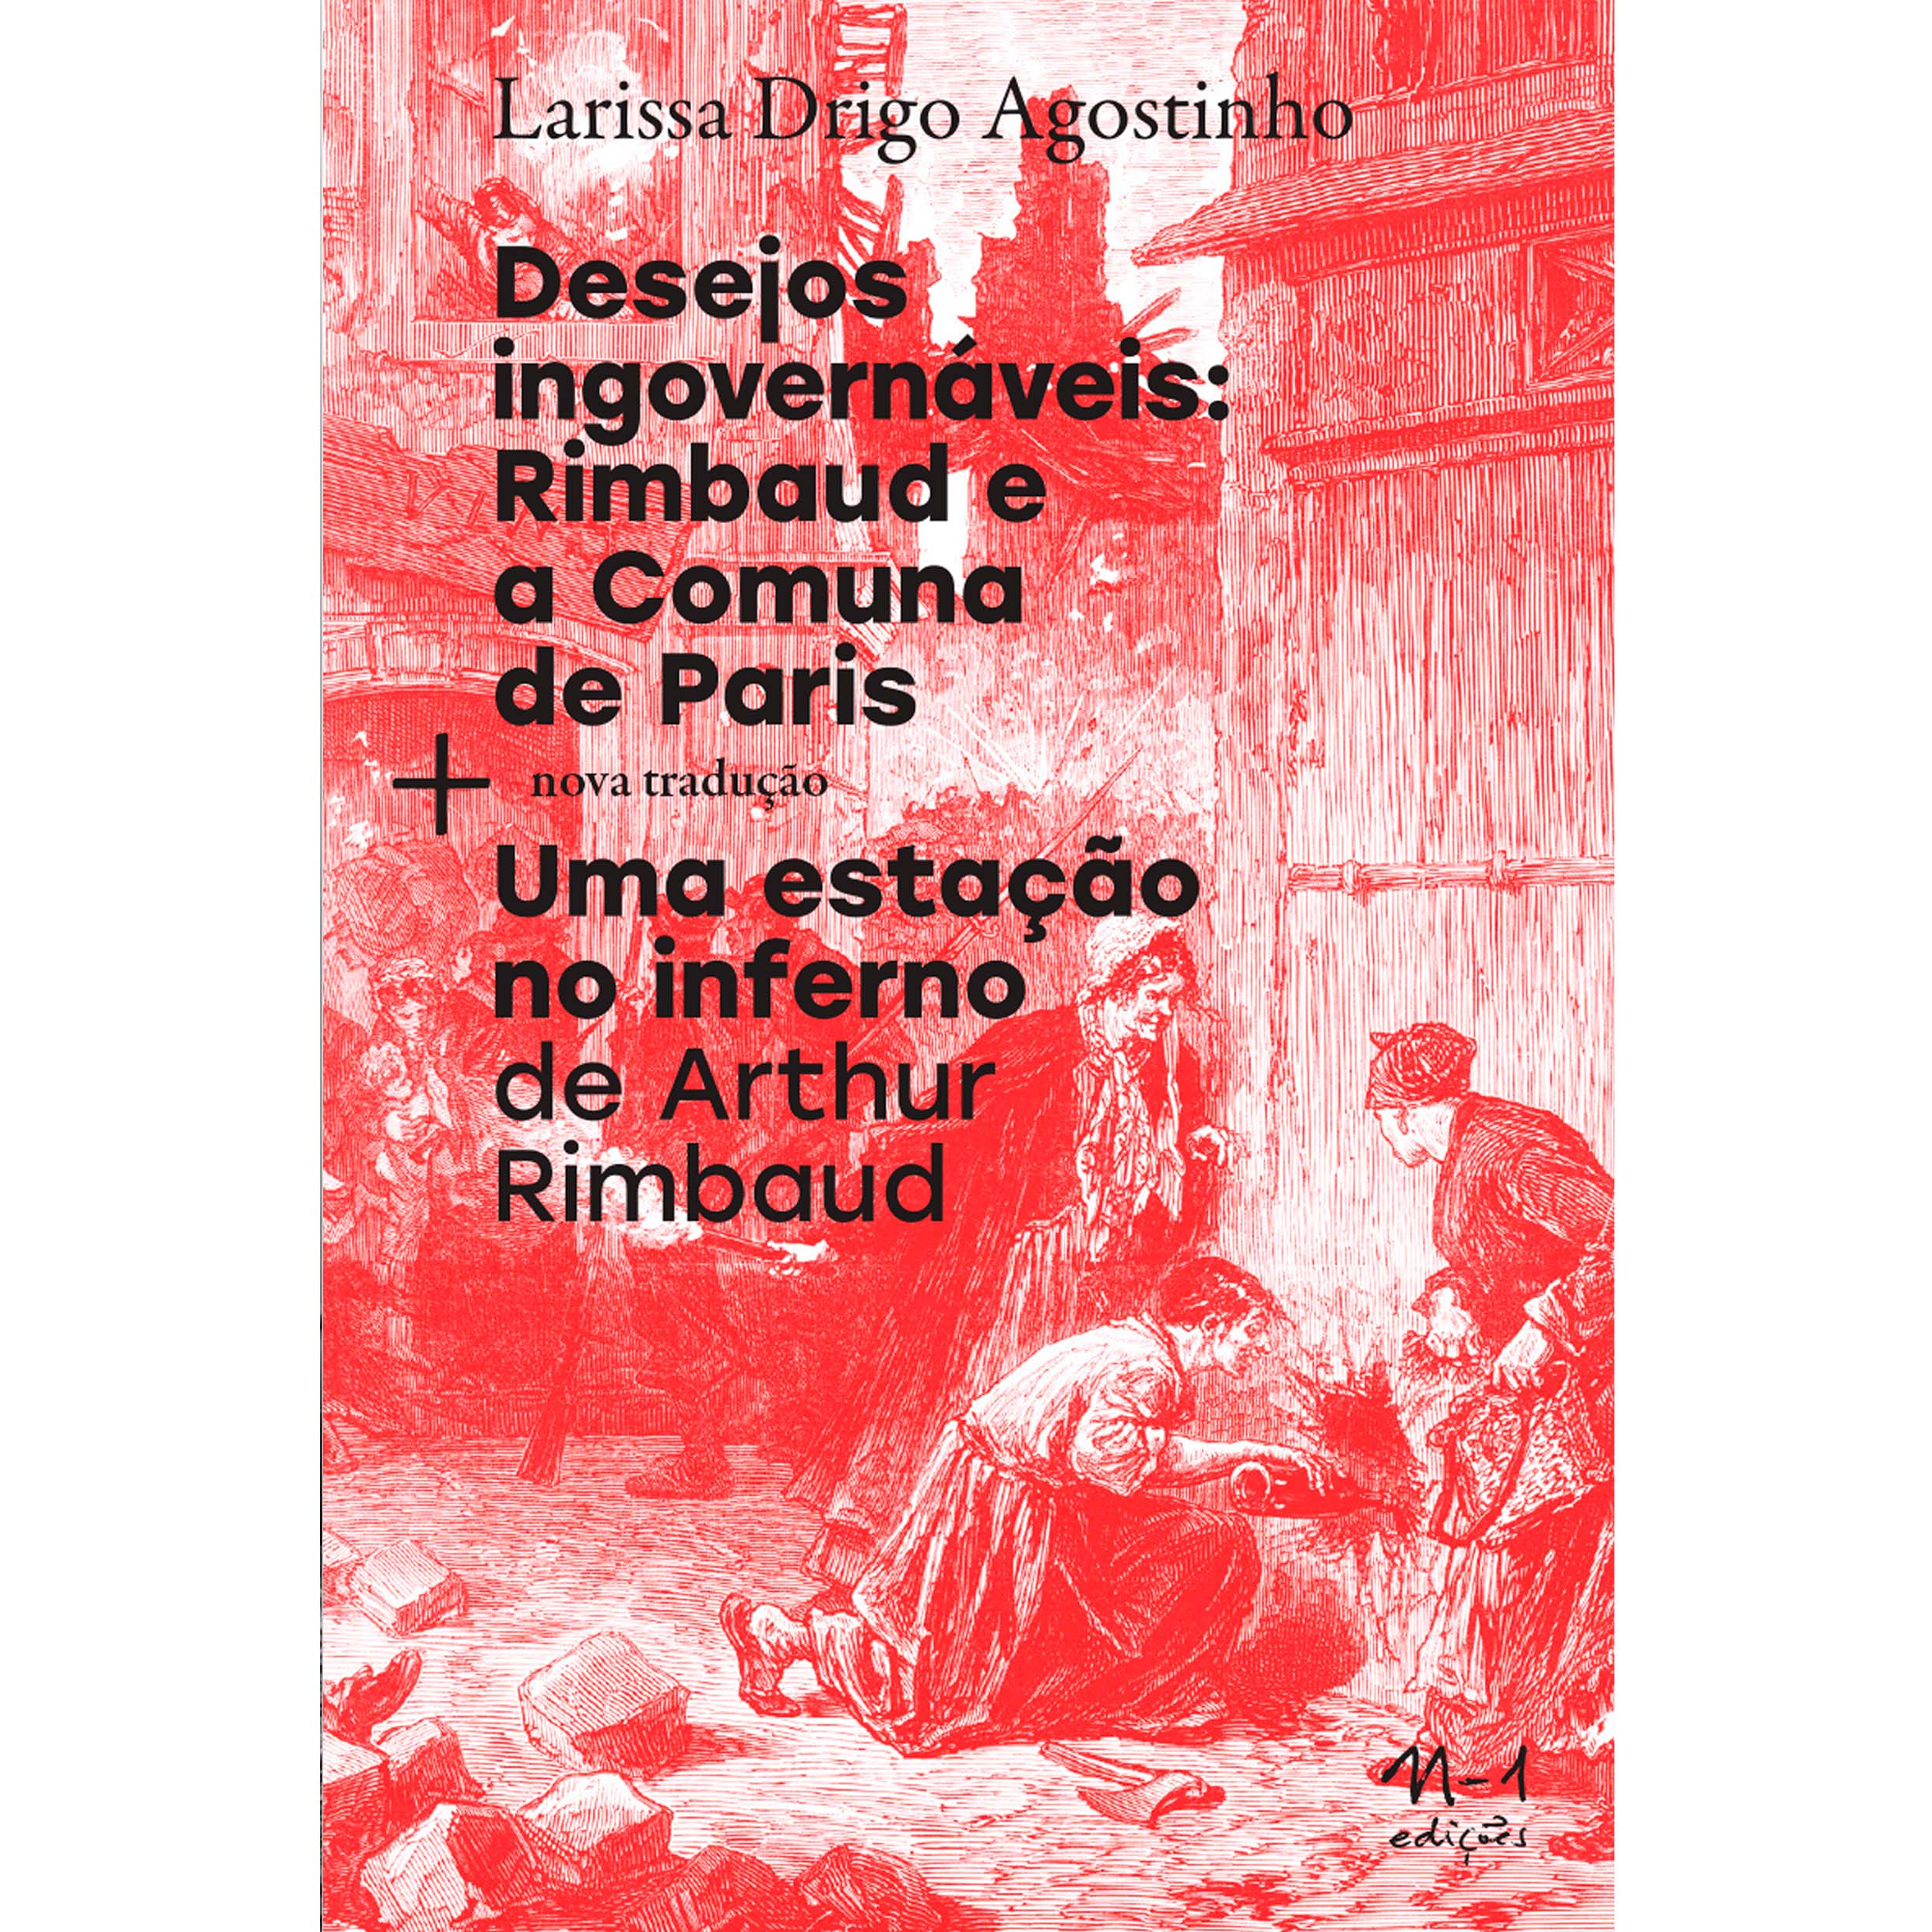
\includegraphics[width=74mm]{./CAPAS/rimbaud.jpg}
\end{center}

\hspace*{-7cm}\hrulefill\hspace*{-7cm}

\medskip

\noindent{}O poema \textit{Uma estação no inferno} é polifônico, atravessado pelas vozes de mulheres loucas, de marginais, de loucos é
porque Rimbaud coloca em questão os alicerces da civilização ocidental, aqueles que tornaram possíveis a colonização e a escravidão, a abnegação e a construção de uma sociedade amante do trabalho e do sacrifício: a moral cristã, o culto da razão, da ciência, do progresso, da ordem e da harmonia.

\vfill

\hspace*{-.4cm}\begin{minipage}[c]{1\linewidth}
\small\textbf{
\hspace*{-.1cm}Editora: n-1\\
Título: Desejos ingovernáveis: Rimbaud e a Comuna de Paris + Uma estação no Inferno\\
Autor: Larissa Drigo Agostinho / Arthur Rimbaud\\
ISBN: 978-65-86941-52-4\\
Páginas: 196\\
Formato: 19x11\,cm\\
Preço: R\$ 68,00\\
}
\end{minipage}

\pagebreak

\begin{center}
\hspace*{.5cm}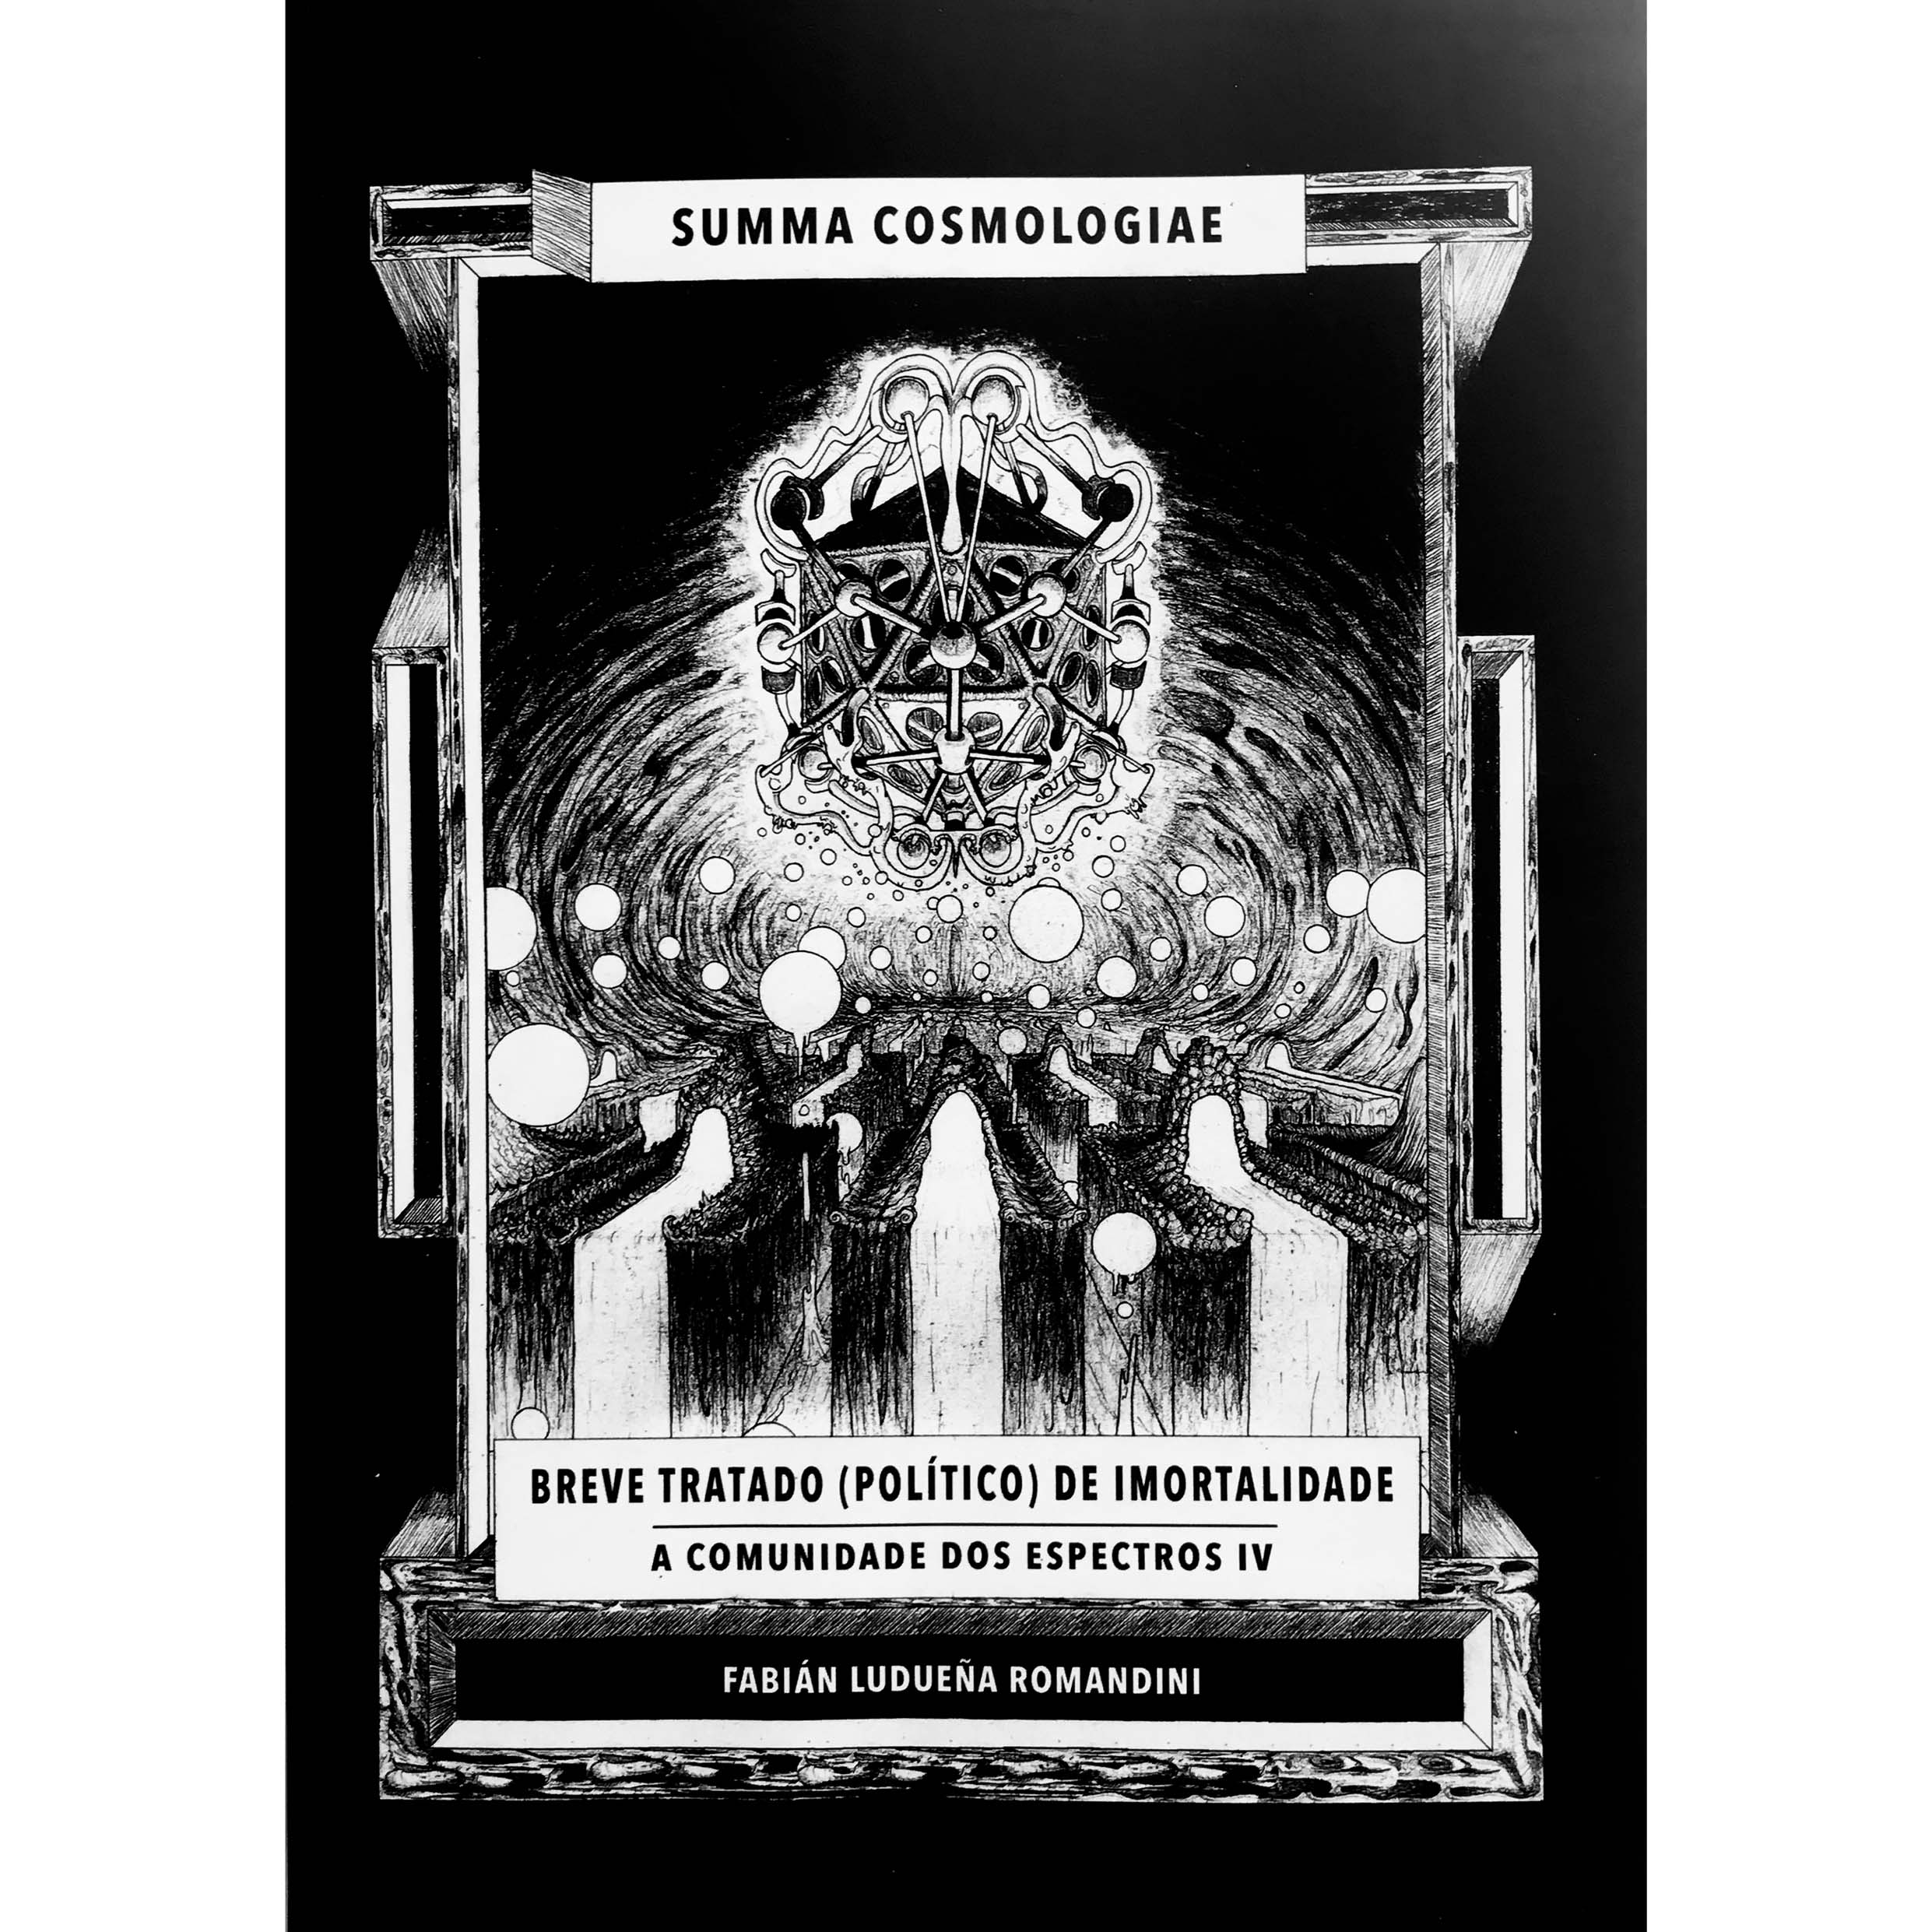
\includegraphics[width=74mm]{./CAPAS/tratado.jpg}
\end{center}

\hspace*{-7cm}\hrulefill\hspace*{-7cm}

\medskip

\noindent{}
\vfill

\hspace*{-.4cm}\begin{minipage}[c]{1\linewidth}
\small\textbf{
\hspace*{-.1cm}Editora: n-1\\
Título: Summa Cosmologiae: Breve tratado (político) de Imortalidade\\
Autor: Fabián Ludueña Romandini\\
ISBN: 978-65-86941-49-4\\
Páginas: 192\\
Formato: 23x16\,cm\\
Preço: R\$ 62,00\\
}
\end{minipage}

\pagebreak

\vspace*{1.5cm}

\noindent{}{\nohyphens{\LARGE{Texto}}}

\bigskip

\hfill{}\scalebox{.8}{AUTOR}

\bigskip
\bigskip
\bigskip

\begin{multicols}{2}
\noindent{}Mussum Ipsum, cacilds vidis litro abertis. Atirei o pau no gatis, per gatis num morreus. Leite de capivaris, leite de mula manquis sem cabeça. Praesent malesuada urna nisi, quis volutpat erat hendrerit non. Nam vulputate dapibus. Suco de cevadiss, é um leite divinis, qui tem lupuliz, matis, aguis e fermentis.

Tá deprimidis, eu conheço uma cachacis que pode alegrar sua vidis. Suco de cevadiss deixa as pessoas mais interessantis. In elementis mé pra quem é amistosis quis leo. Quem num gosta di mim que vai caçá sua turmis!

Viva Forevis aptent taciti sociosqu ad litora torquent. Mauris nec dolor in eros commodo tempor. Aenean aliquam molestie leo, vitae iaculis nisl. Posuere libero varius. Nullam a nisl ut ante blandit hendrerit. Aenean sit amet nisi. Vehicula non. Ut sed ex eros. Vivamus sit amet nibh non tellus tristique interdum.

Em pé sem cair, deitado sem dormir, sentado sem cochilar e fazendo pose. Detraxit consequat et quo num tendi nada. Pra lá , depois divoltis porris, paradis. Per aumento de cachacis, eu reclamis.

Quem manda na minha terra sou euzis! A ordem dos tratores não altera o pão duris. Paisis, filhis, espiritis santis. Aenean aliquam molestie leo, vitae iaculis nisl.

Diuretics paradis num copo é motivis de denguis. Mais vale um bebadis conhecidiss, que um alcoolatra anonimis. Sapien in monti palavris qui num significa nadis i pareci latim. Admodum accumsan disputationi eu sit. Vide electram sadipscing et per.

Manduma pindureta quium dia nois paga. Interagi no mé, cursus quis, vehicula ac nisi. Praesent vel viverra nisi. Mauris aliquet nunc non turpis scelerisque, eget. Casamentiss faiz malandris se pirulitá.

Quem num gosta di mé, boa gentis num é. Si num tem leite então bota uma pinga aí cumpadi! Todo mundo vê os porris que eu tomo, mas ninguém vê os tombis que eu levo! Cevadis im ampola pa arma uma pindureta.

\vspace{\baselineskip}

{\small\fakereceipt{
\noindent{}Diuretics paradis num copo é motivis de denguis. Mais vale um bebadis conhecidiss, que um alcoolatra anonimis. Sapien in monti palavris qui num significa nadis i pareci latim. Admodum accumsan disputationi eu sit. Vide electram sadipscing et per.
}}

\vspace{\baselineskip}

Mussum Ipsum, cacilds vidis litro abertis. Atirei o pau no gatis, per gatis num morreus. Leite de capivaris, leite de mula manquis sem cabeça. Praesent malesuada urna nisi, quis volutpat erat hendrerit non. Nam vulputate dapibus. Suco de cevadiss, é um leite divinis, qui tem lupuliz, matis, aguis e fermentis.

Tá deprimidis, eu conheço uma cachacis que pode alegrar sua vidis. Suco de cevadiss deixa as pessoas mais interessantis. In elementis mé pra quem é amistosis quis leo. Quem num gosta di mim que vai caçá sua turmis!

Viva Forevis aptent taciti sociosqu ad litora torquent. Mauris nec dolor in eros commodo tempor. Aenean aliquam molestie leo, vitae iaculis nisl. Posuere libero varius. Nullam a nisl ut ante blandit hendrerit. Aenean sit amet nisi. Vehicula non. Ut sed ex eros. Vivamus sit amet nibh non tellus tristique interdum.

Em pé sem cair, deitado sem dormir, sentado sem cochilar e fazendo pose. Detraxit consequat et quo num tendi nada. Pra lá , depois divoltis porris, paradis. Per aumento de cachacis, eu reclamis.

Quem manda na minha terra sou euzis! A ordem dos tratores não altera o pão duris. Paisis, filhis, espiritis santis. Aenean aliquam molestie leo, vitae iaculis nisl.

Diuretics paradis num copo é motivis de denguis. Mais vale um bebadis conhecidiss, que um alcoolatra anonimis. Sapien in monti palavris qui num significa nadis i pareci latim. Admodum accumsan disputationi eu sit. Vide electram sadipscing et per.

Manduma pindureta quium dia nois paga. Interagi no mé, cursus quis, vehicula ac nisi. Praesent vel viverra nisi. Mauris aliquet nunc non turpis scelerisque, eget. Casamentiss faiz malandris se pirulitá.

Quem num gosta di mé, boa gentis num é. Si num tem leite então bota uma pinga aí cumpadi! Todo mundo vê os porris que eu tomo, mas ninguém vê os tombis que eu levo! Cevadis im ampola pa arma uma pindureta.

\bigskip

\noindent{}\textcolor{gray}{\footnotesize\slsc{\textls[-15]{Texto tal tal e tal.}}}
\end{multicols}


\pagebreak
\pagestyle{n-1cat}

\begin{multicols}{2}
\begin{enumerate}
\raggedright\nohyphens{
\item Potências do tempo, \textbf{David Lapoujade}
\item Declaração, \textbf{Antonio Negri; Michael Hardt}
\item Manifesto contrassexual, \textbf{Beatriz Preciado}
\item O aracniano e outros textos, \textbf{Fernand Deligny}
\item Deleuze, os movimentos aberrantes, \textbf{David Lapoujade}
\item Aos nossos amigos, \textbf{Comitê Invisível}
\item Teoria King Kong, \textbf{Virginie Despentes}
\item Guattari: Confrontações / Conversas com Kuniichi Uno e Laymert Garcia dos Santos
\item Quando e como eu li Foucault, \textbf{Antonio Negri}
\item O avesso do niilismo, \textbf{Peter Pál Pelbart}
\item A missão, \textbf{Heiner Müller}
\item William James, a construção da experiência, \textbf{David Lapoujade}
\item Nietzsche -- O bufão dos deuses, \textbf{Maria Cristina Franco Ferraz}
\item Impressões de Michel Foucault, \textbf{Roberto Machado}
\item Fabulações do corpo japonês, \textbf{Christine Greiner}
\item As existências mínimas, \textbf{David Lapoujade}
\item Hegel e o Haiti, \textbf{Susan Buck-Morss}
\item Brazuca, negão e sebento, \textbf{Jean-Christophe Goddard}
\item Motim e destituição agora, \textbf{Comitê Invisível}
\item Crítica da razão negra, \textbf{Achille Mbembe}
\item Testo junkie, \textbf{Paul B. Preciado}
\item O universo inacabado, \textbf{Mario Novello}
\item Cartas e outros textos, \textbf{Gilles Deleuze}
\item Nietzsche e a filosofia, \textbf{Gilles Deleuze}
\item Hijikata tatsumi, \textbf{Kuniichi Uno}
\item Spartakus, \textbf{Furio Jesi}
\item Agamben: por uma ética da vergonha e do resto, \textbf{Oswaldo Giacóia Junior}
\item UPP -- A redução da favela em três letras, \textbf{Marielle Franco}
\item Cinco dias em março, \textbf{Toshiki Okada}
\item Os vagabundos eficazes, \textbf{Fernand Deligny}
\item O enigma da revolta, \textbf{Michel Foucault}
\item Arqueofeminismo
\item Contribuição para a guerra em curso, \textbf{Tiqqun}
\item Ética bixa, \textbf{Paco Vidarte}
\item Ensaios do assombro, \textbf{Peter Pál Pelbart}
\item Metafísicas canibais, \textbf{Eduardo Viveiros de Castro}
\item O governo do homem endividado, \textbf{Maurizio Lazzarato}
\item Leituras do corpo no Japão, \textbf{Christine Greiner}
\item Pragmatismo pulsional, \textbf{João Perci Schiavon}
\item Ruptura, \textbf{Centelha}
\item Às voltas com Lautréamont, \textbf{Laymert Garcia dos Santos}
\item Afrotopia, \textbf{Felwine Sarr}
\item Fascismo ou revolução?, \textbf{Maurizio Lazzarato}
\item Corpos que importam, \textbf{Judith Butler}
\item Somos nosso cérebro?, \textbf{Francisco Ortega; Fernando Vidal}
\item Ritornelos, \textbf{Félix Guattari}
\item Contracultura, entre a curtição e o experimental, \textbf{Celso Favarett}
\item Necropolítica, \textbf{Achille Mbembe}
\item Esferas da inssureição: notas para uma vida não cafetinada, \textbf{Suely Rolnik}

}
\end{enumerate}
\end{multicols}

\pagebreak